
\subsection{Run 7 optical modifications}\label{run-7-optical-modifications}

For Run 7 in the white room on Level 3 our EO test setup had a few differences from the Run 6 setup in IR2 at SLAC. One difference was that we were not able to use the CCOB Narrow/Thin beam because we did not have the resources to configure it. As
such, the majority of the testing was done with the CCOB Wide Beam
projector\citep{2024SPIE13103E..0WU}. We did obtain an additional projector, the 4K projector, partway through Run 7 that will be discussed later. With the CCOB Wide Beam,
we used a cone attached to the L1 cover as well as a shroud to create a
dark environment (Fig.~\ref{fig:LSSTCam_config}).

\begin{figure}[htbp]
\centering
    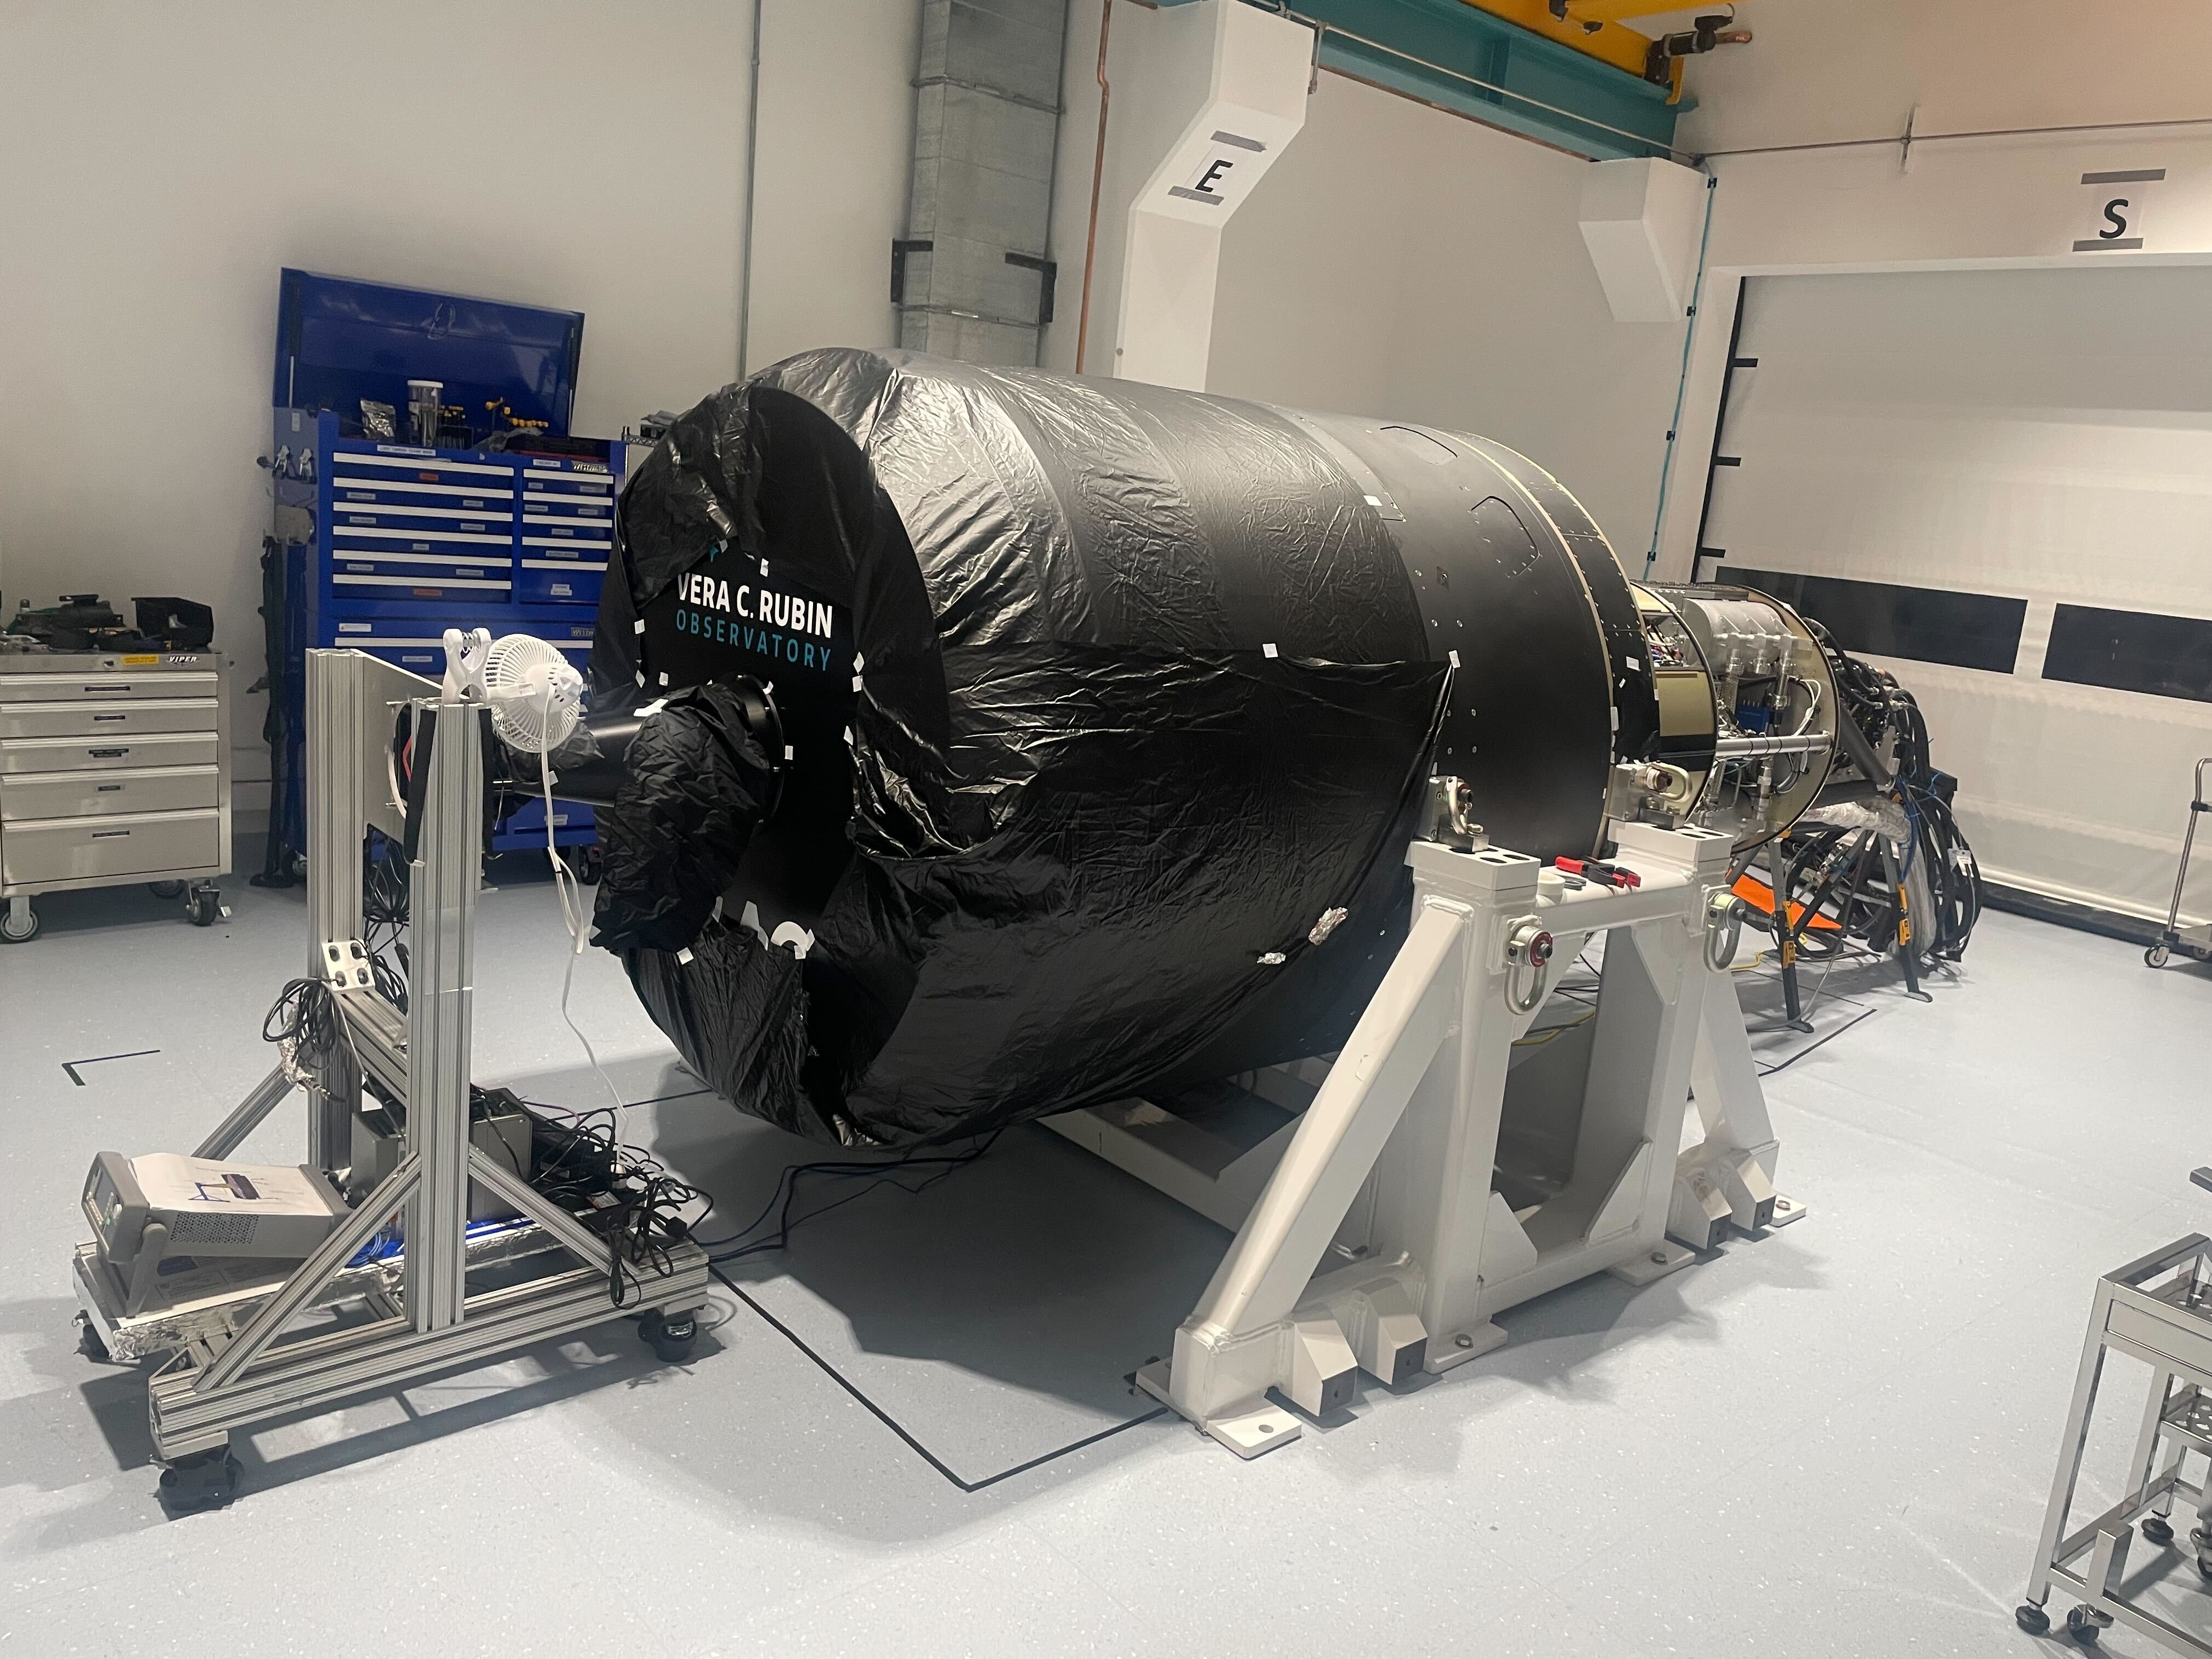
\includegraphics[width=0.6\textwidth]{figures/Camera_Shroud.jpg} 
    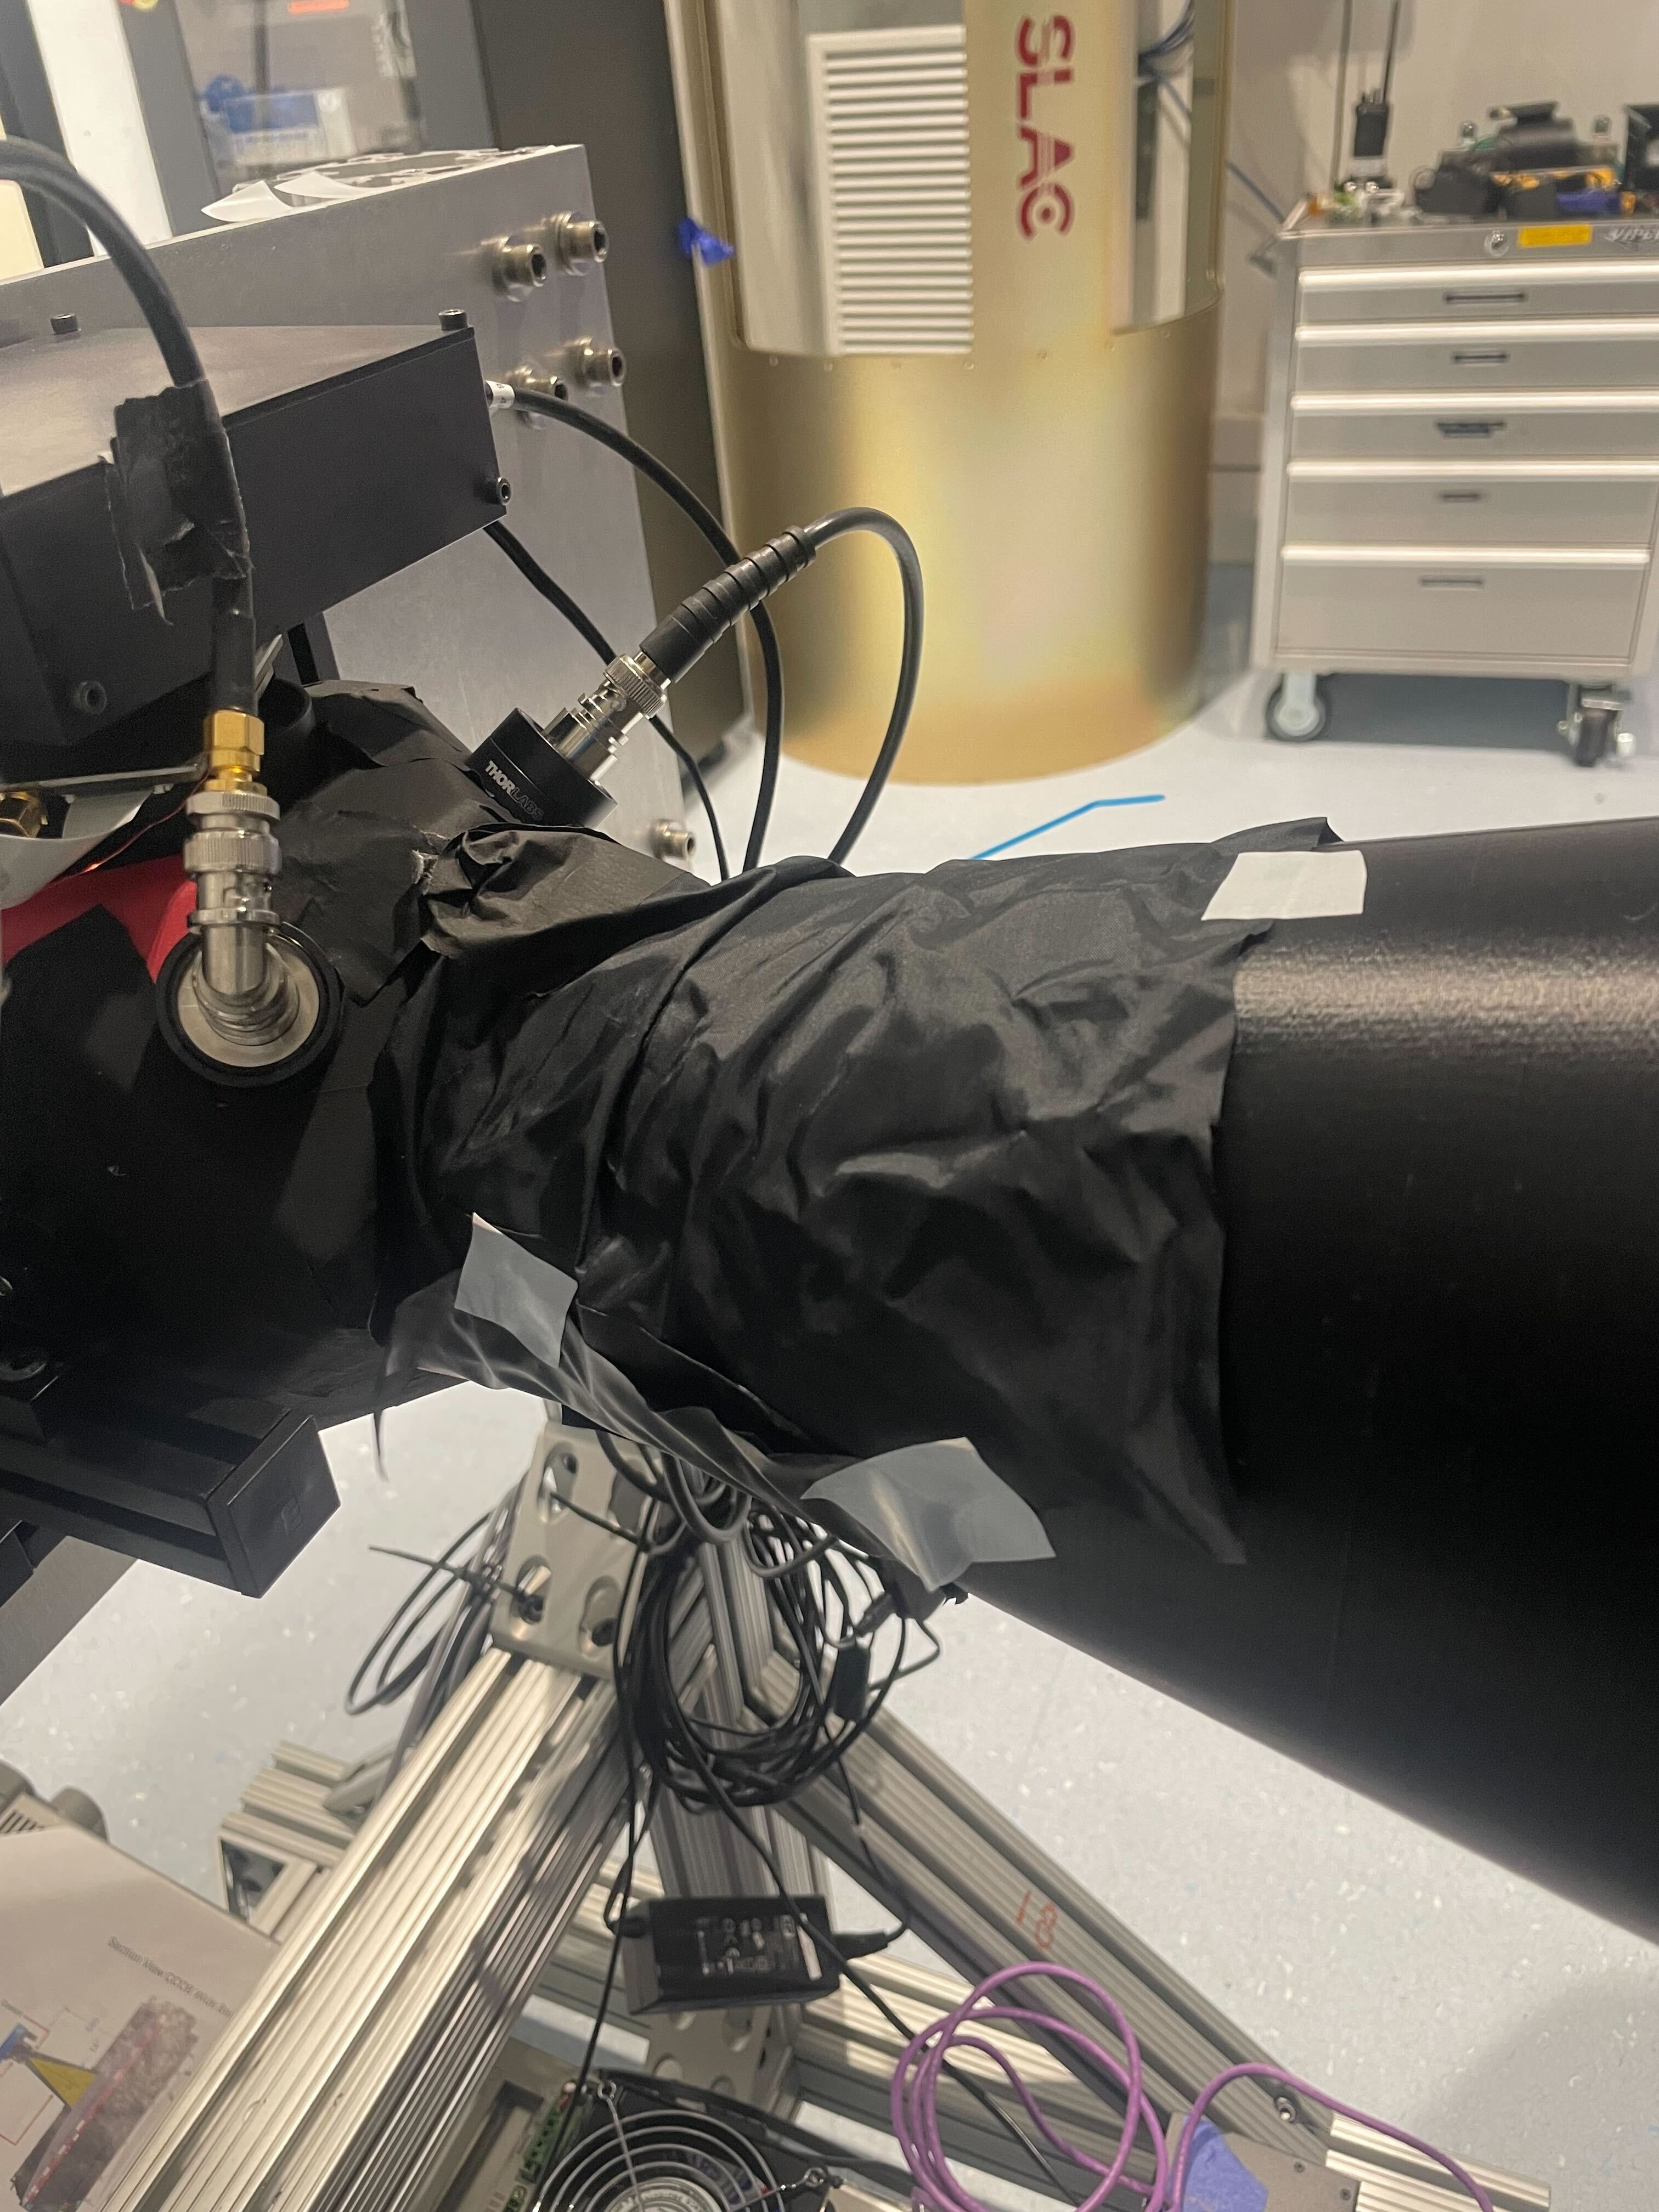
\includegraphics[width=0.35\textwidth]{figures/CCOB_Wide_Shroud.jpg} \\
\caption{(left) Final shroud configuration of LSST Camera in Level 3 to reduce light leaks. (right) CCOB Wide Beam attached to the cone and shrouded.}
\label{fig:LSSTCam_config}
\end{figure}

This allowed us to operate on Level 3 with a dark current of \textless0.1 ADU/sec with the shutter open. The initial setup of the CCOB Wide Beam projector was the same as for Run 6, with a minimal ND filter (10\%) attached to a C-mount lens. One difference was that the f/stop of the lens was changed from 2.6 to 1.6 (fully open). This was done to try to reduce the effect of the `weather' and the `CMB pattern' two effects that we found in Run 6 and were found to be due to our projection setup (see \citet{2024arXiv241113386B}). While changing  the f/stop  did reduce the weather pattern, it also caused a much steeper illumination roll-off across the focal plane (see Figures \ref{fig:roll-off} and \ref{fig:Rolloff_FP}). We evaluated the weather pattern and illumination roll-off relative to Run 6.


To both reduce the effects of the `weather' and `CMB' but retain uniform illumination across the focal plane, we installed a diffuser in the cone attached to L1. Figure~\ref{fig:diffuser} shows the placement of the diffuser within the cone.  The diffuser used is a $60^o$ diffusing angle unmounted sheet from Edmunds Optics.

\begin{figure}[ht]
\centering
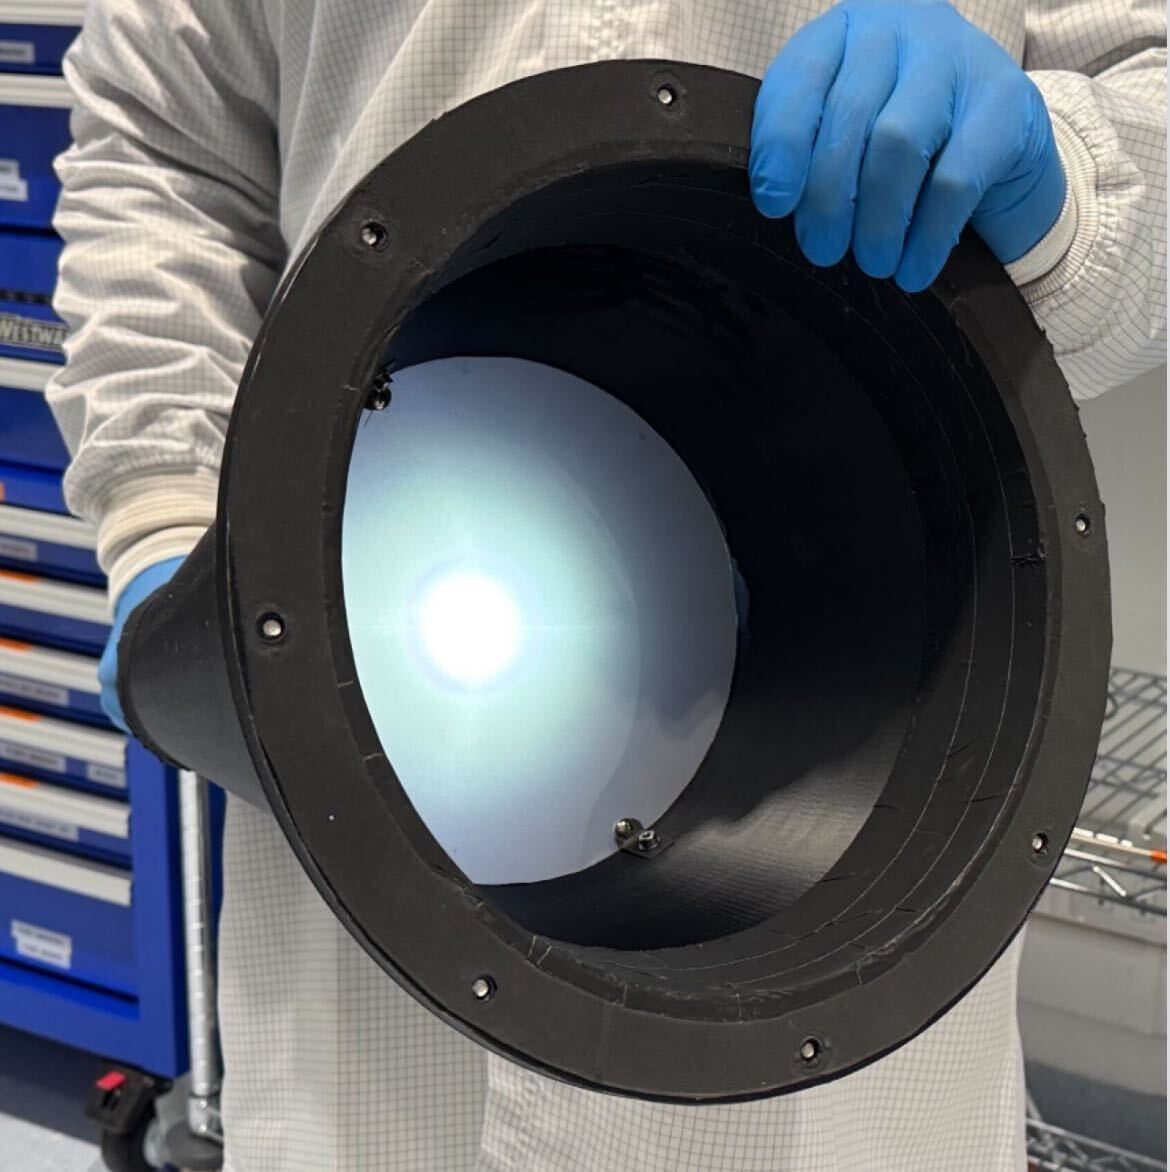
\includegraphics[width=0.6\textwidth]{figures/Diffuser.jpg}
\caption{Diffuser installed into the light cone.}
\label{fig:diffuser}
\end{figure}

We found that the diffuser greatly reduced the `weather' (Fig.~\ref{fig:weather}) and eliminated the CMB pattern and more uniformly illuminated the focal plane (Fig.~\ref{fig:roll-off}), and removed the extreme roll-off (Fig. \ref{fig:roll-off} and Fig. \ref{fig:Rolloff_FP}) with a penalty of decreasing the overall illumination by roughly 35\% even though we fully opened the f-stop.


\begin{figure}[htbp]
\centering
\begin{minipage}{0.45\textwidth}
    \centering
    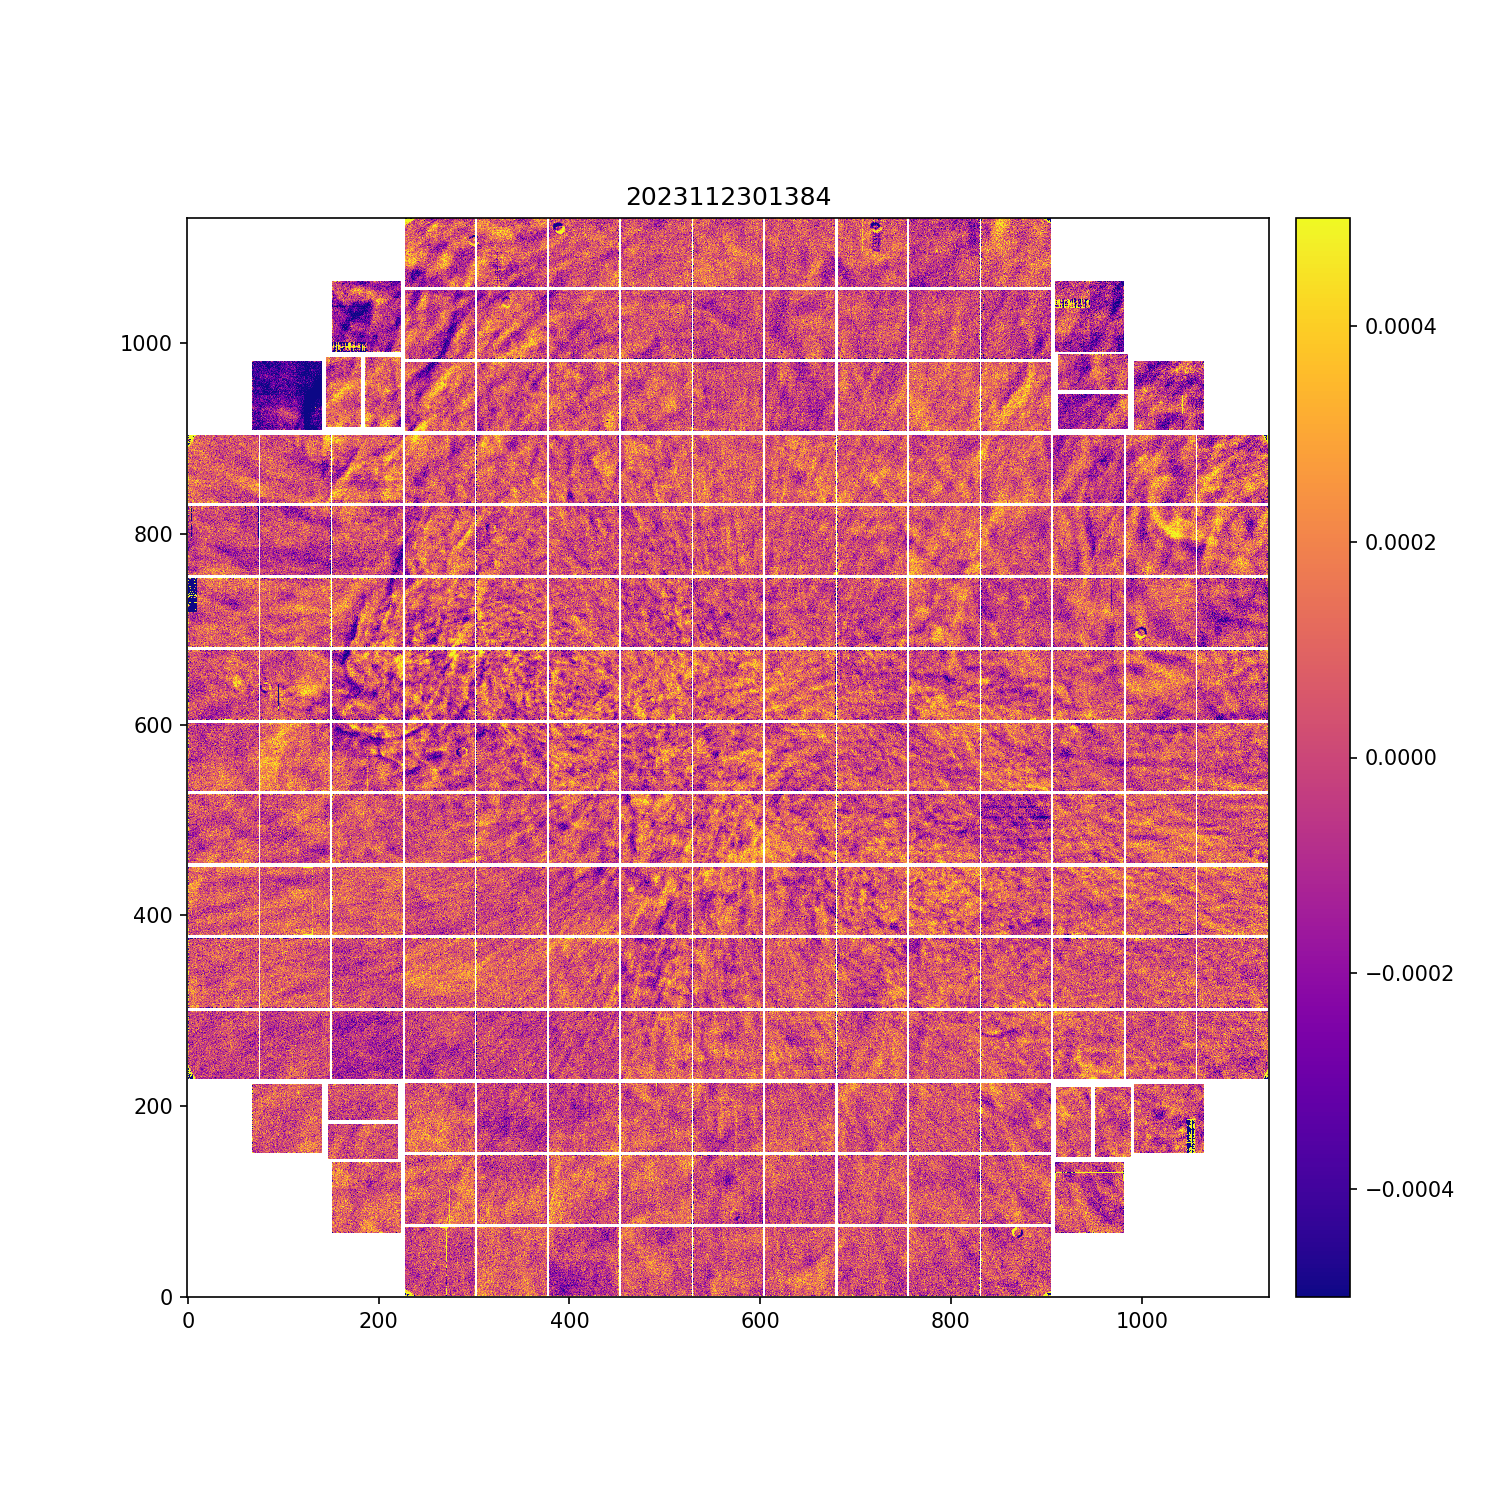
\includegraphics[width=\linewidth]{figures/Run6_Weather.png}
%    \caption{Full focal plane image showing the fractional difference in Run 6.}
\end{minipage}
%\hfill
\begin{minipage}{0.5\textwidth}
    \centering
    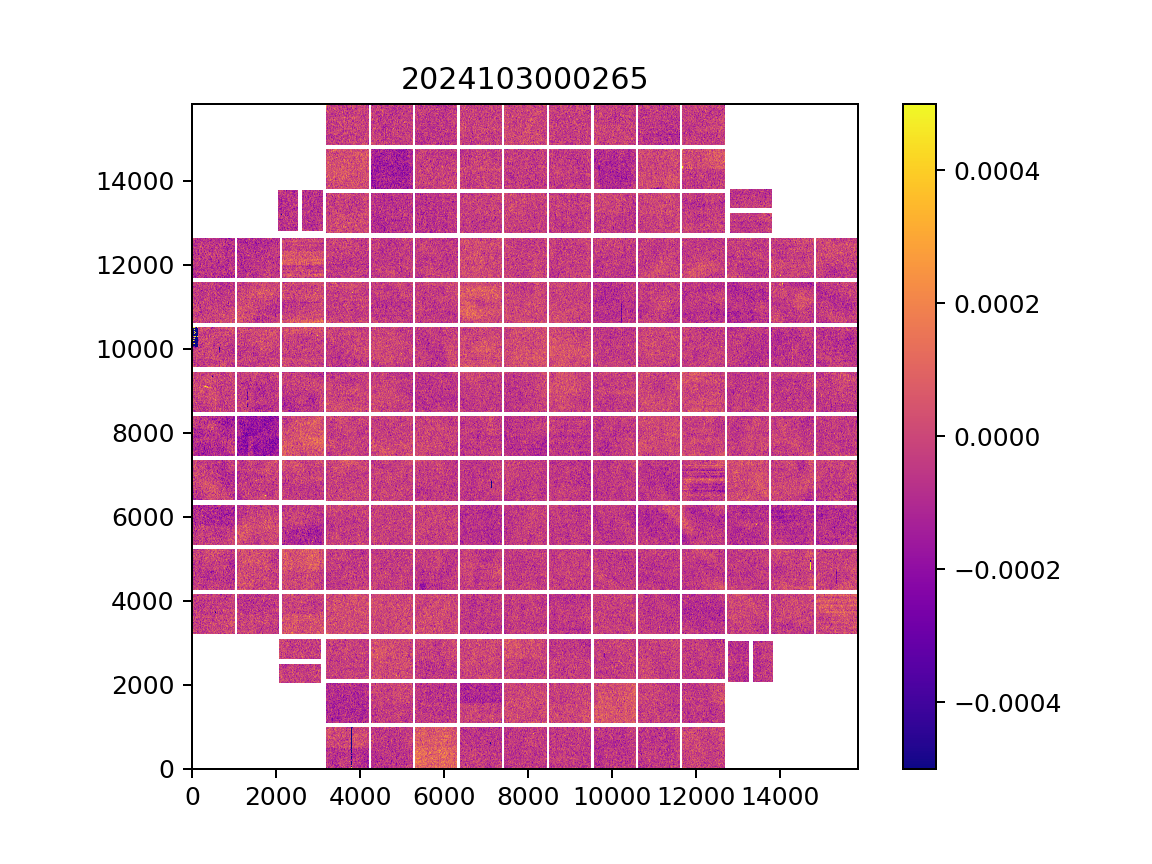
\includegraphics[width=\linewidth]{figures/Run7_WeatherDiffuser.png}
\end{minipage}    
    \caption{Full focal plane fractional difference of images for Run 6 (left) and Run 7 (right).}

\label{fig:weather}
\end{figure}

\begin{figure}[htbp]
\centering
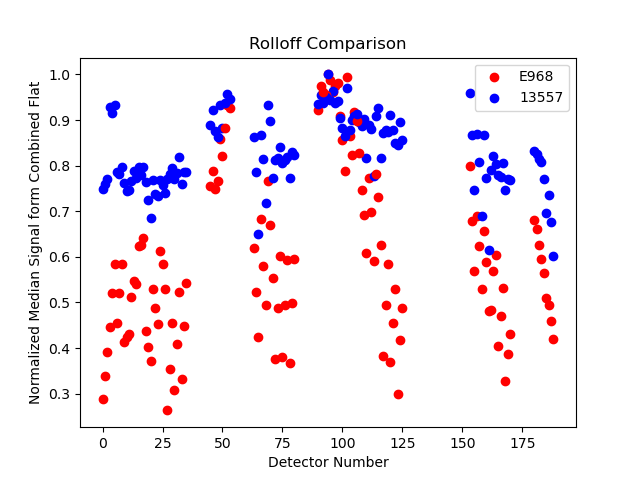
\includegraphics[width=0.48\textwidth]{figures/Run7_Illumination.png}
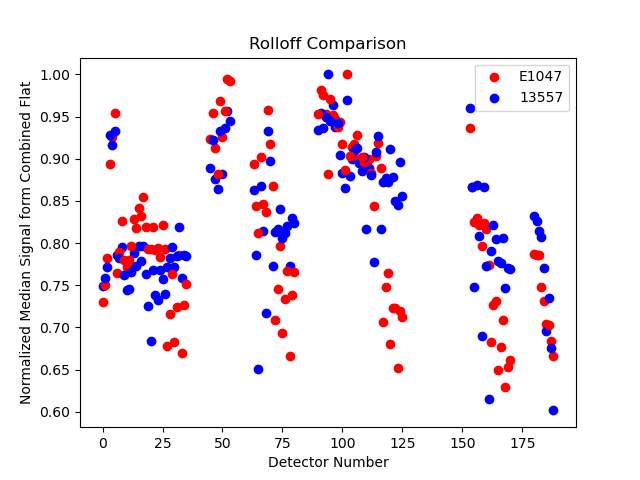
\includegraphics[width=0.48\textwidth]{figures/Run7_DiffuserIllumination.png}
\caption{(left) Illumination across the focal plane from Run 7 without the diffuser (E968) as compared to Run 6. (right) Illumination across the focal plane from Run 7 with the diffuser (E1047) as compared to Run 6.}
\label{fig:roll-off}
\end{figure}

\begin{figure}[ht]
    \centering
    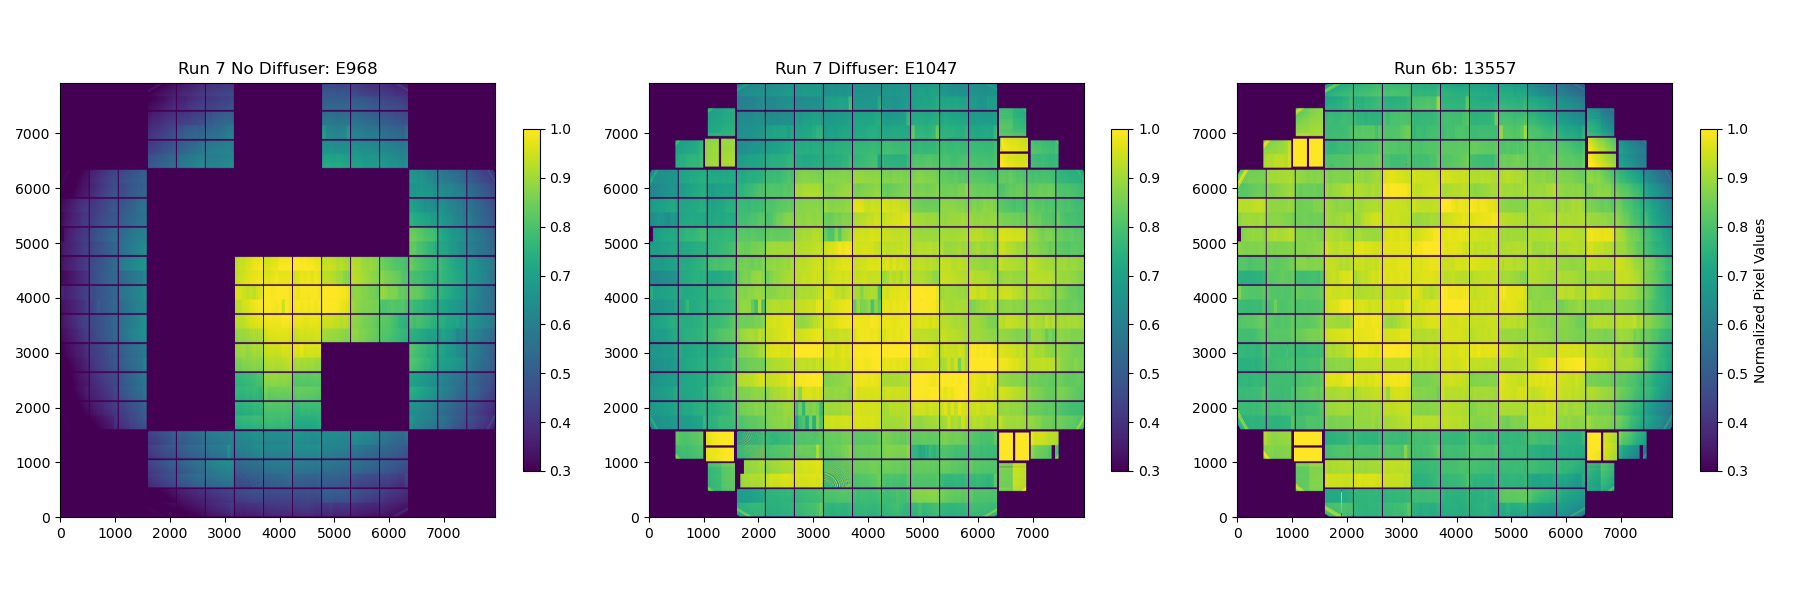
\includegraphics[width=0.95\linewidth]{figures/Rolloff_FP.png}
    \caption{Combined flat images from three different runs that show the roll-off of the CCOB Wide Beam with Run 7 data without the diffuser and with the projector aperture open (left), Run 7 data with the diffuser and projector aperture closed (middle), and Run 6 without the diffuser but the projector aperture closed (right). The pixels are normalized and the left figure is missing detectors as we were still in the process turning them off when doing this test.}
    \label{fig:Rolloff_FP}
\end{figure}


The diffuser was installed for all B protocol and PTC runs (see Sec. \ref{sec:reverification}) moving forward, being taken out only for pinhole projection runs and when using the 4K projector.

\subsection{Projector spots}\label{projector-spots}
The addition to the projectors used for EO testing was a 4K projector (Epson LS11000 LCD), similar to those used in conference rooms. This projector was first tested at SLAC and arrived at the observatory about halfway through Run 7. It was used primarily as a spot projector, as the pinhole filter was not available at that time because of the Filter Exchange System was temporarily inoperable. The projector has an advantage, instead, as it could illuminate all 3206 amplifiers instead of just the 21 illuminated by the
pinhole projector. Figure \ref{fig:SpotProjector_L3_FP} shows both the setup of the projector on Level 3 and an example of a spot image and the spots across the focal plane. Since the projector does not have fast illumination control, we primarily used the LSST camera main shutter instead of any flashing of the light source (e.g., as we did with the LEDs of the CCOB Wide Beam). One downside that was found was that the projector illuminated the entire focal plane at some background level, not just the spot regions. The background illumination also had structure that changed with time and could not be easily subtracted. Figure \ref{fig:SpotProjector_Spots} shows an example of a spot image of just one detector as well as a zoomed in image of a single spot which highlights the background structure. The resulting contrast between the spot and the background was only about a factor of 6. Changing the spot shape to large rectangles for crosstalk
measurements increased the contrast ratio to 30. Examples of the rectangles can be seen in Figure \ref{fig:SpotProjector_Rect}. Though the contrast was much improved, there was still a background structure as can be seen in the saturated image of the figure.

\begin{figure}[htbp]
\centering
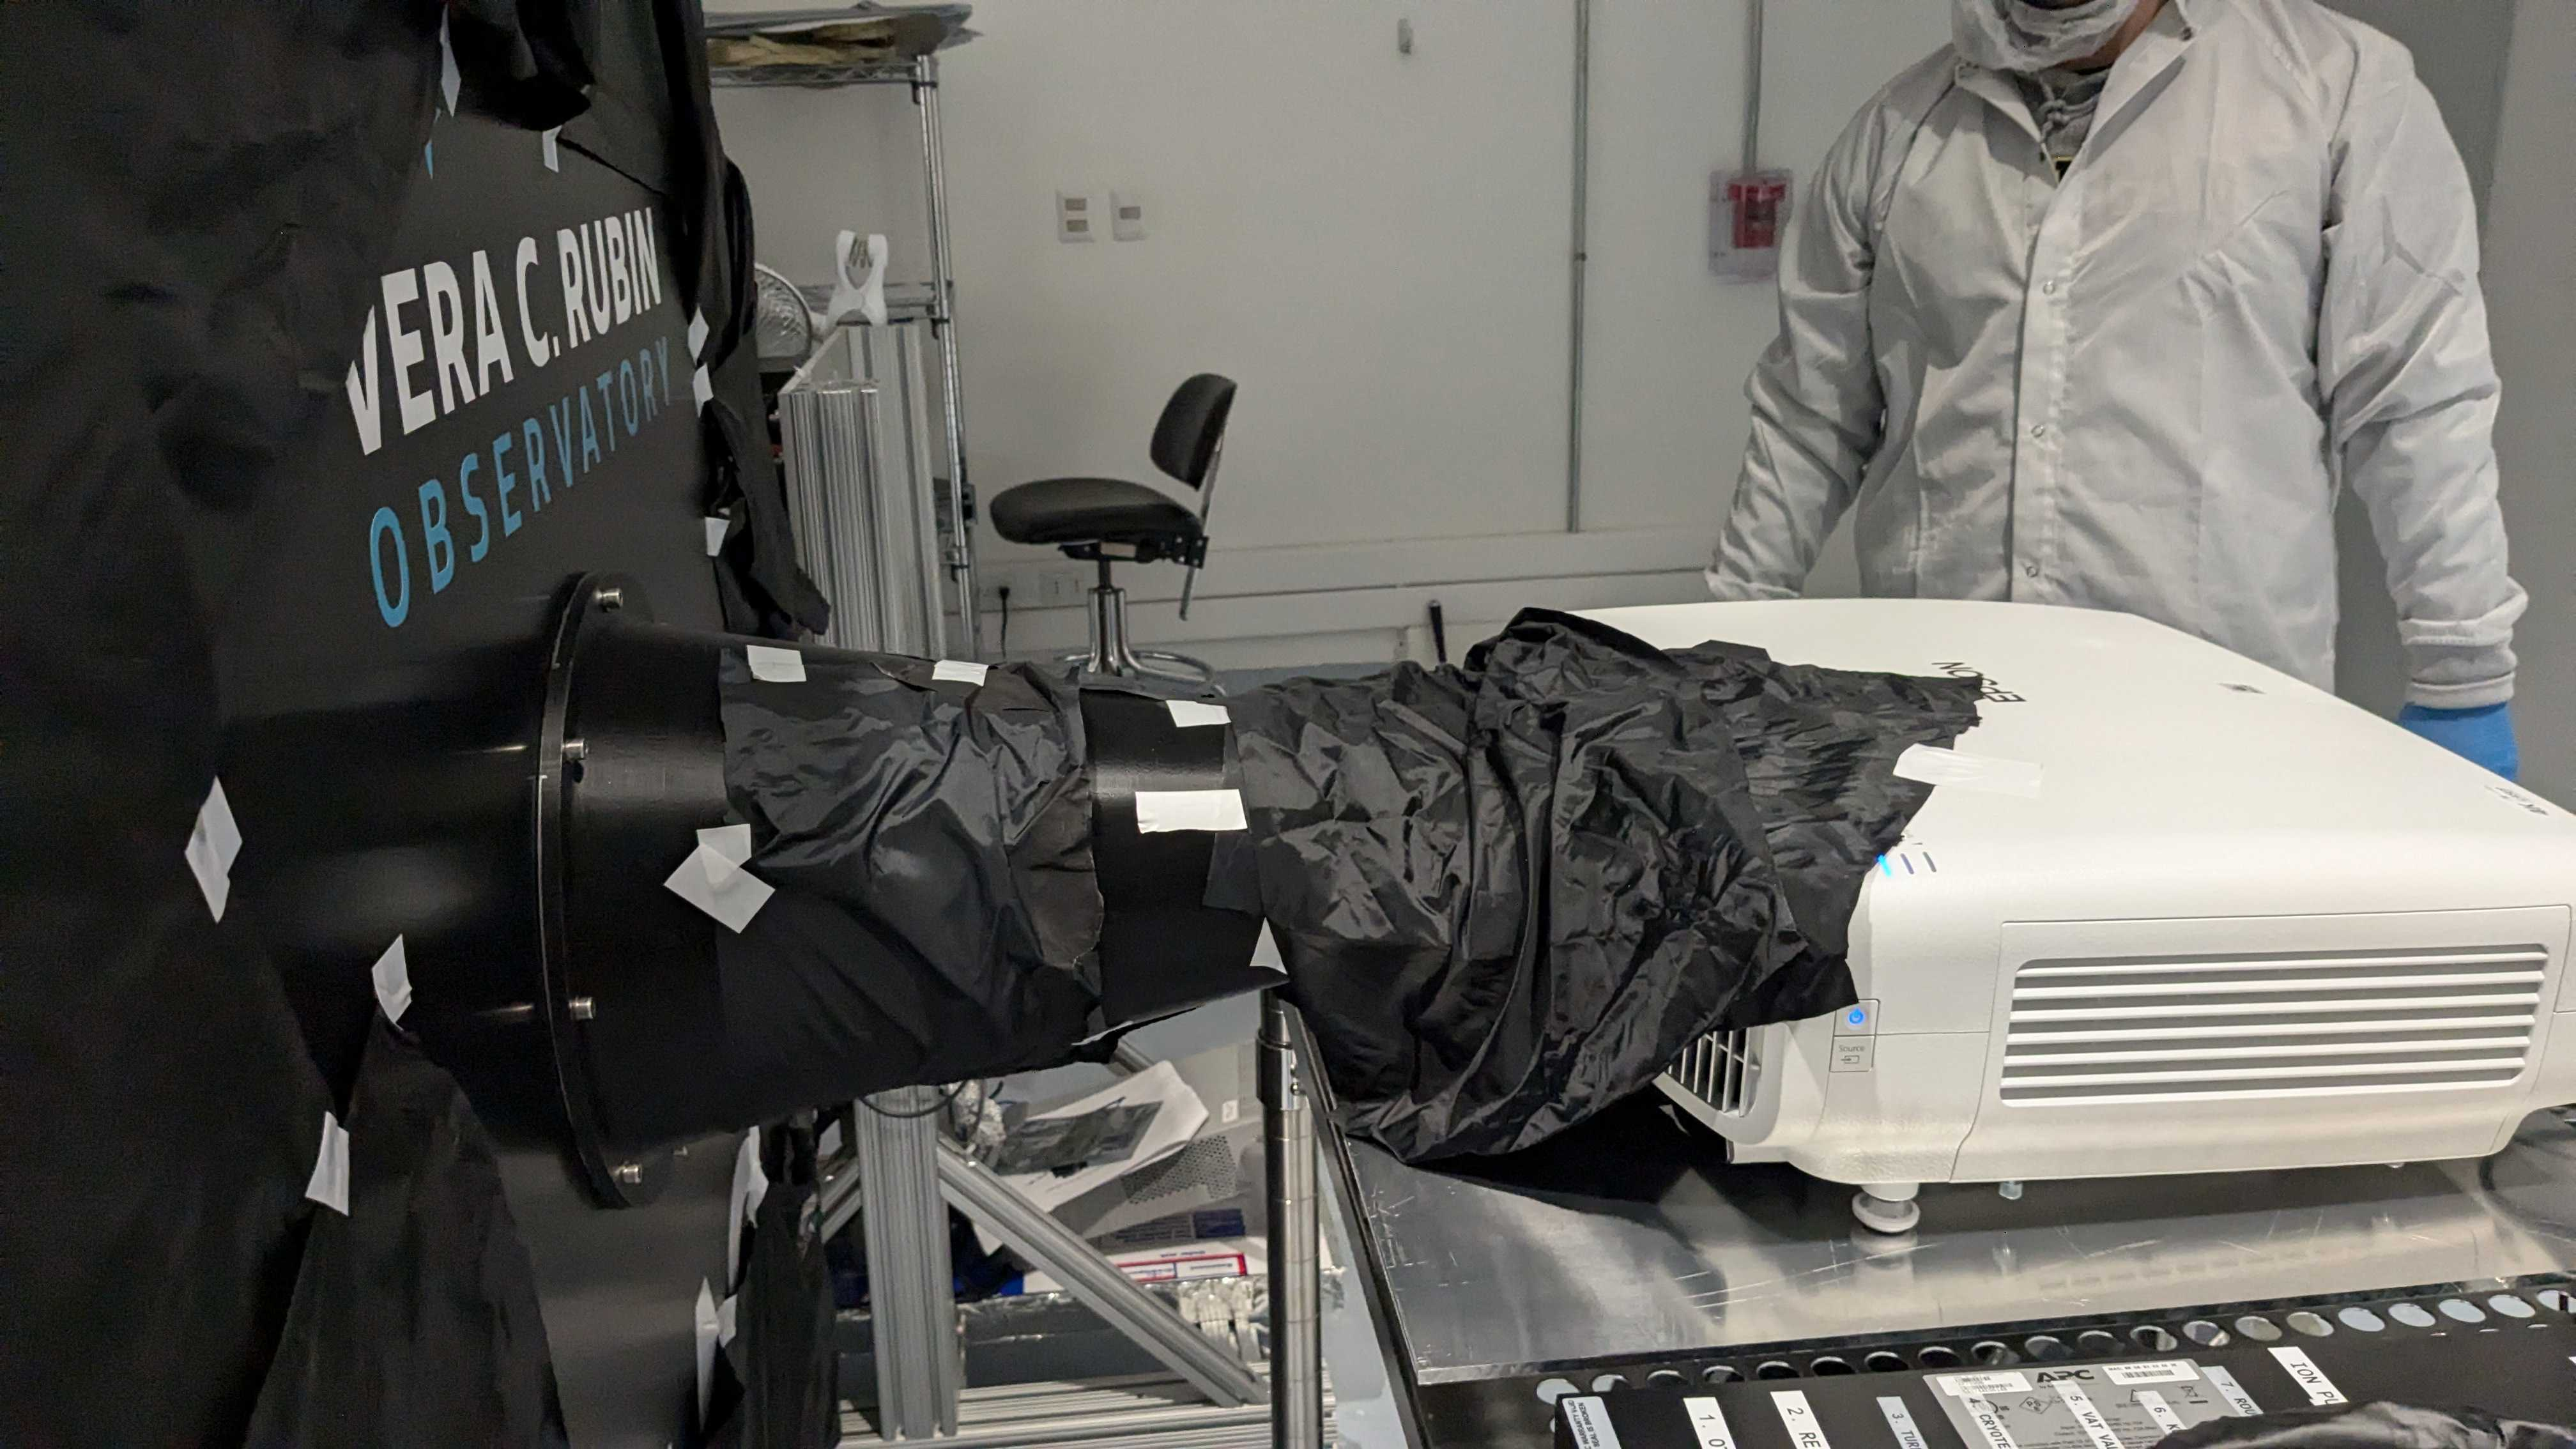
\includegraphics[width=0.48\textwidth]{figures/SpotProjector_Level3.jpg}
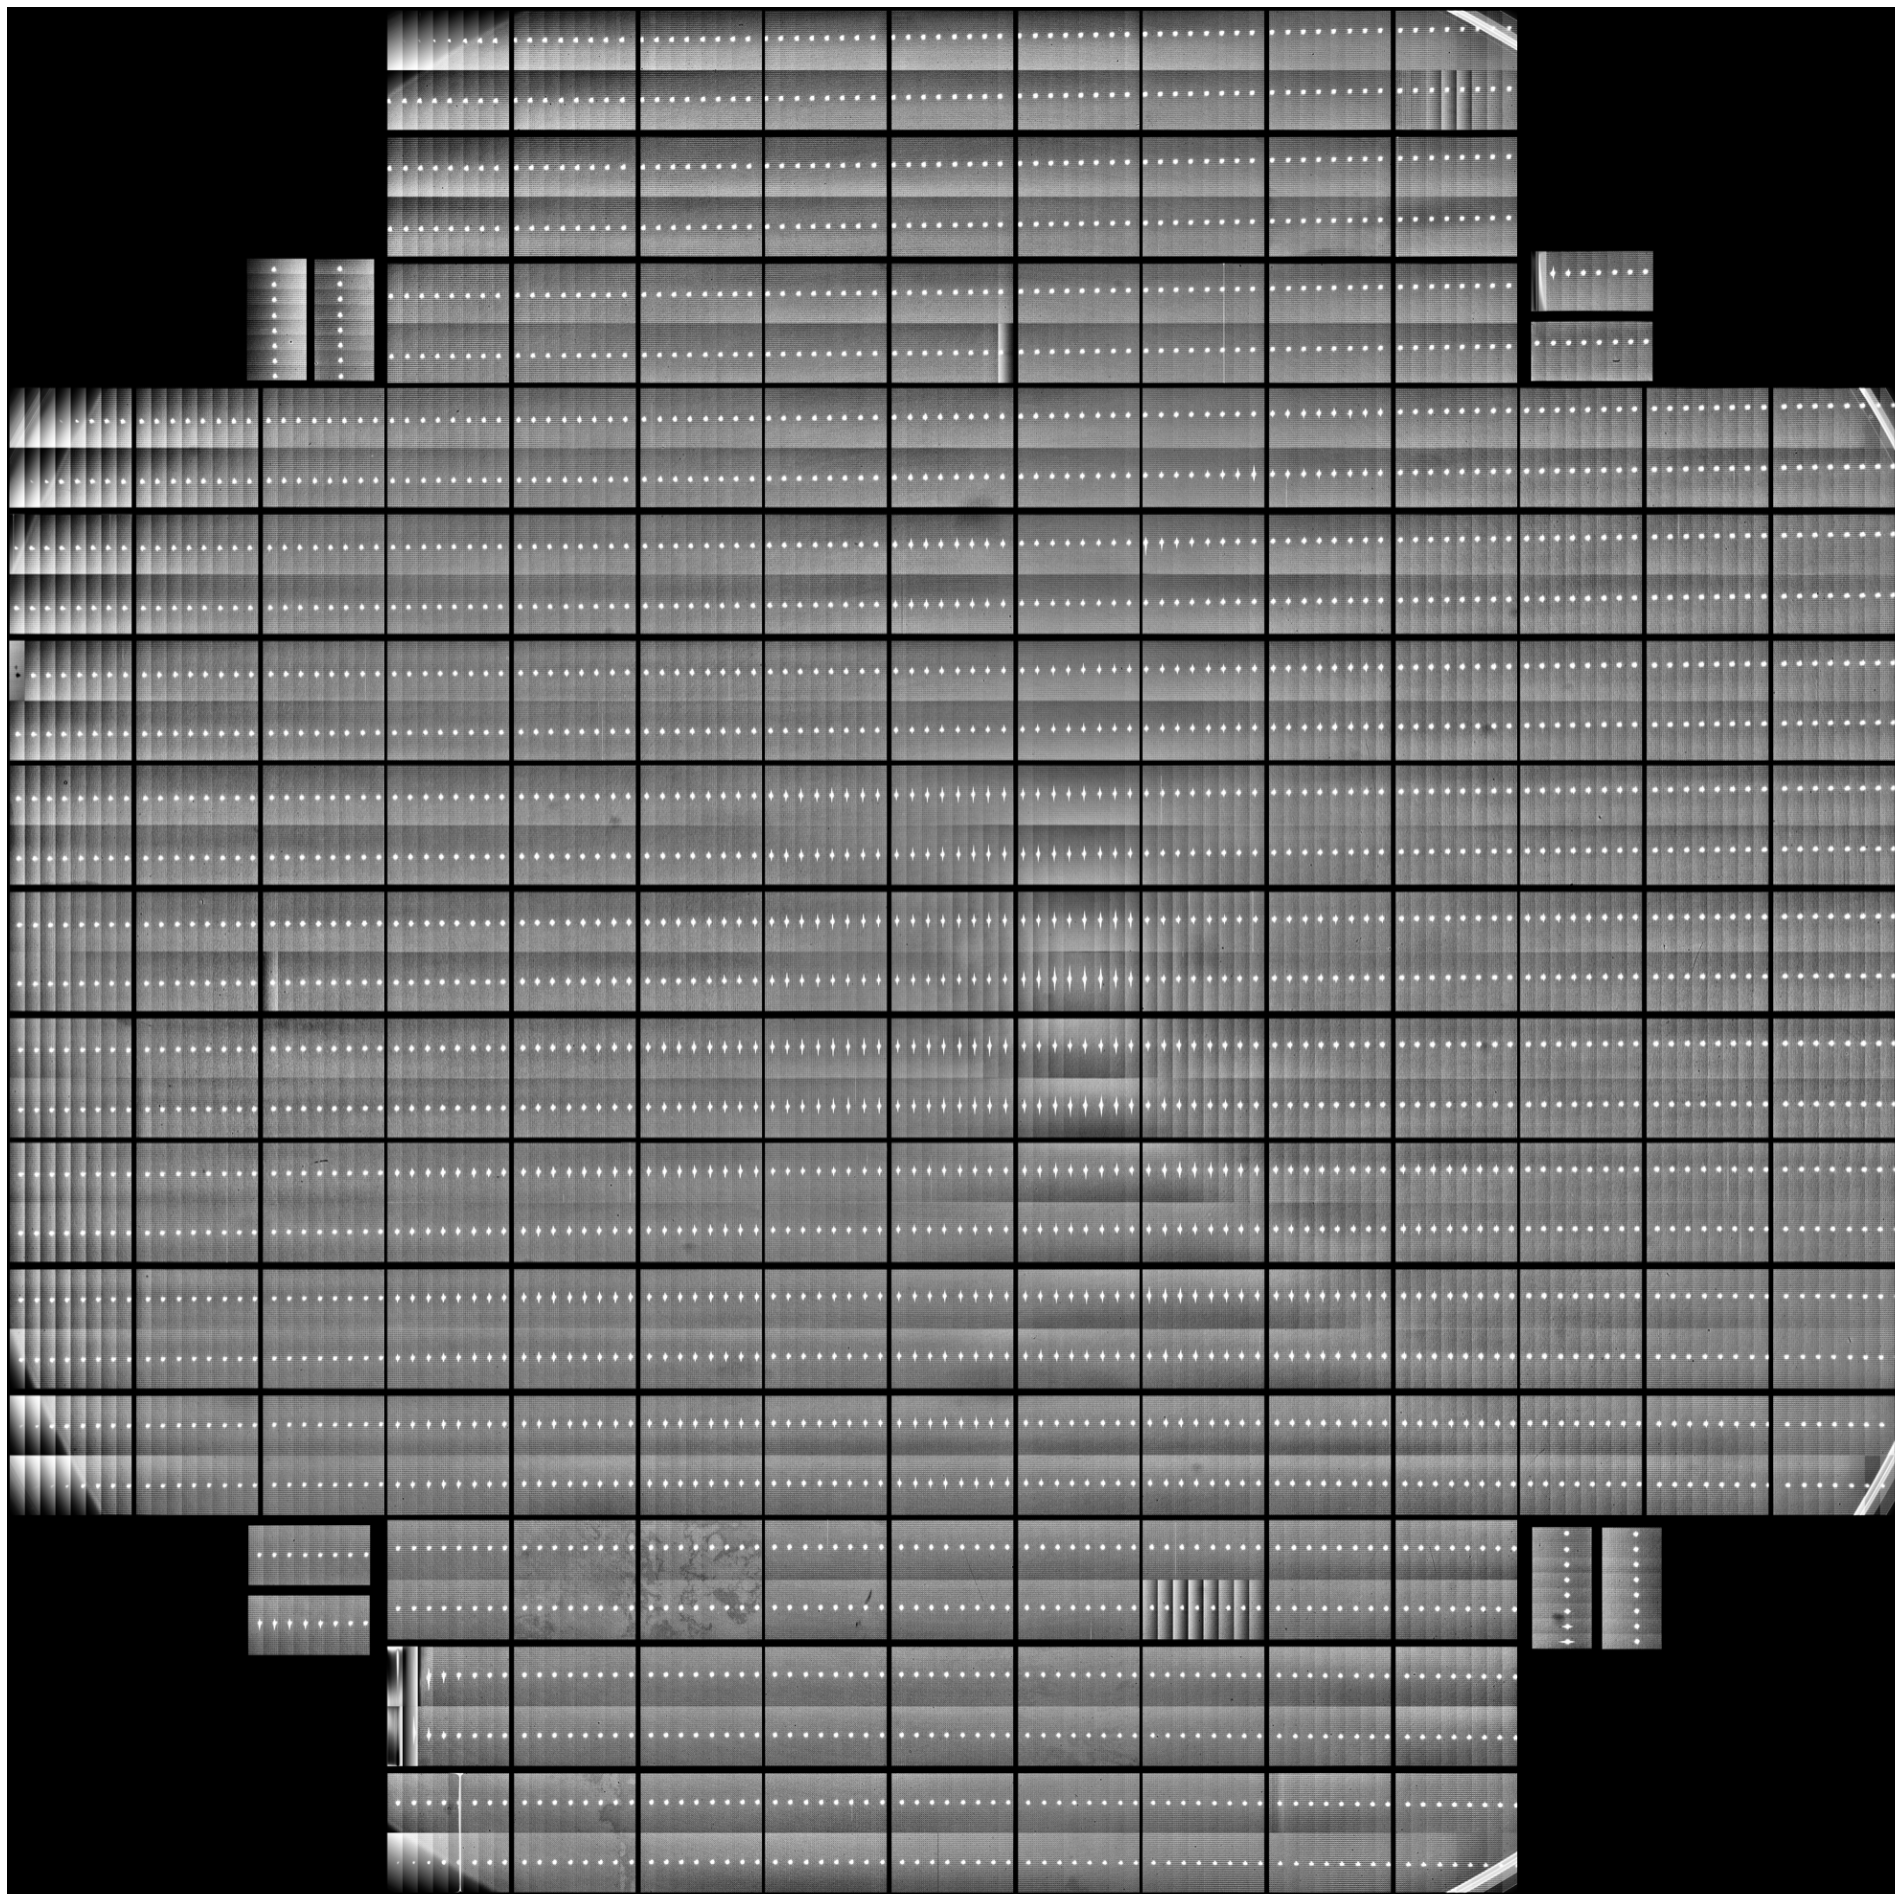
\includegraphics[width=0.48\textwidth]{figures/SpotProjector_FP.png}
\caption{(left) The spot projector set up on Level 3. (right) An example of an image taken with the spot projector with all the amplifiers containing a spot.}
\label{fig:SpotProjector_L3_FP}
\end{figure}

\begin{figure}[htbp]
\centering
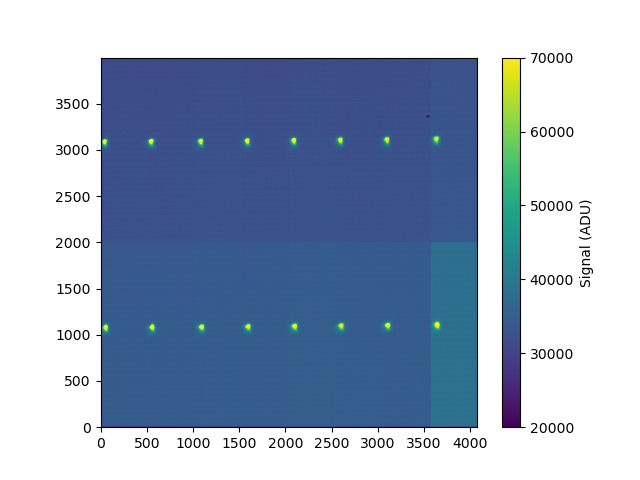
\includegraphics[width=0.48\textwidth]{figures/Spot_Detector_Ex.png}
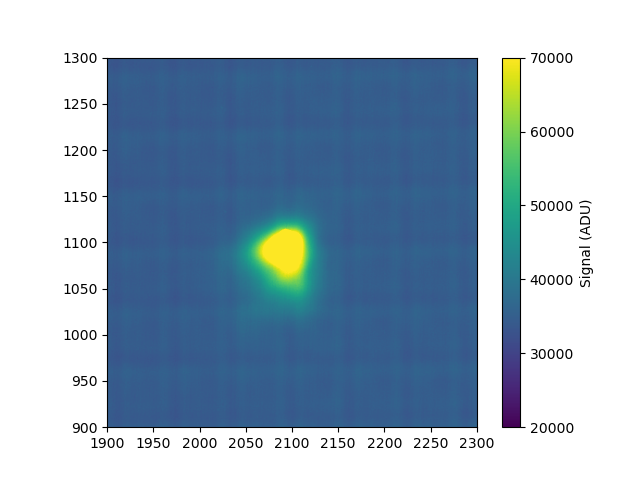
\includegraphics[width=0.48\textwidth]{figures/Spot_Spot_Ex.png}
\caption{(left) Example of a spot image zooming into a single detector. (right) Example of a spot image zooming further into a single spot. In both the images, there is a clear background structure caused by the projector.}
\label{fig:SpotProjector_Spots}
\end{figure}

\begin{figure}[htbp]
\centering
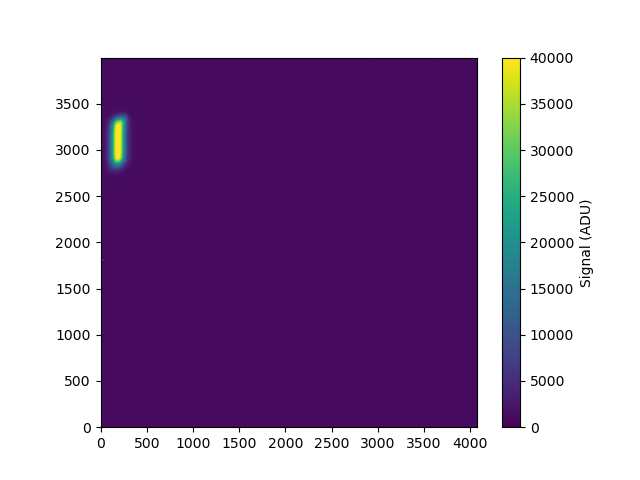
\includegraphics[width=0.32\textwidth]{figures/Rectange_Detector_Ex.png}
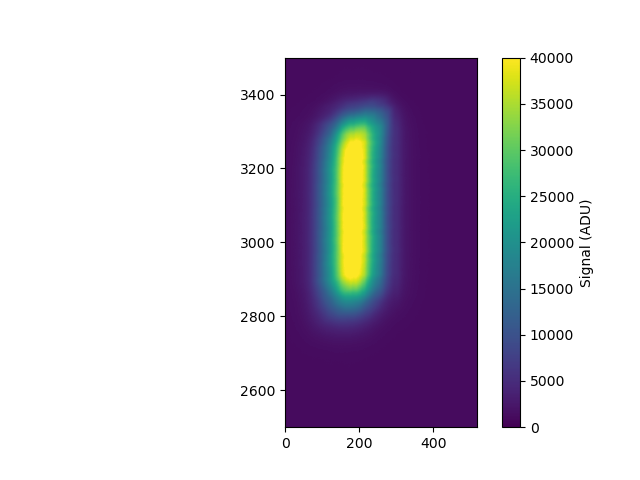
\includegraphics[width=0.32\textwidth]{figures/Rectange_Spot_Ex.png}
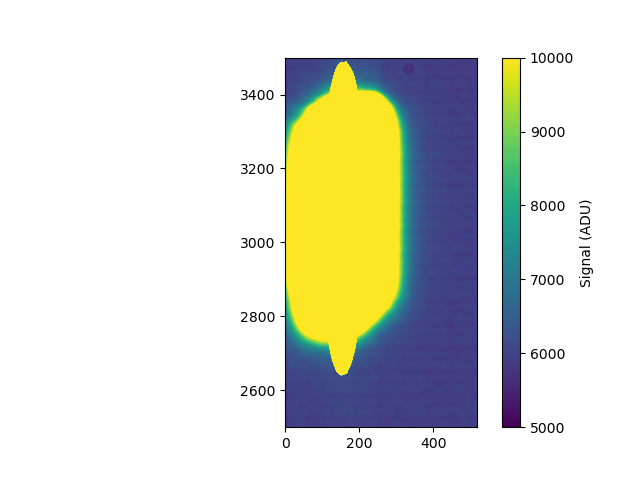
\includegraphics[width=0.32\textwidth]{figures/Rectange_Spot_Sat.png}
\caption{(left) Example of a spot image that utilized the rectangle shape, zoomed into a single detector (left), zoomed into the spot (middle) and zoomed into the spot with a saturated image to highlight the background pattern caused by the projector (right).}
\label{fig:SpotProjector_Rect}
\end{figure}

This section describes the spots and rectangle patterns used for tests with the 4K
projector.

\begin{itemize}
\tightlist
\item  Projector background
\item  Spots on many amps
\item  Spots on one amp
\item  Optical setup
\end{itemize}

\subsection{Dark current and light
leaks}\label{dark-current-and-light-leaks}

%This section describes dark current and light leaks in Run 7 testing.

\subsubsection{Light leak mitigation with shrouding the camera
body}\label{light-leak-mitigation-with-shrouding-the-camera-body}

One of the first tests we attempted with LSST Camera was measuring dark
current and sources of light leaks in the camera body. Before beginning we covered gaps between the L1 cover and the gaskets with tape, in accessible locations . Figure \ref{fig:L1_Gaps} shows the gaps that we could see between L1 and its cover. The inaccessible locations were later covered with shroud.

\begin{figure}[htbp]
\centering
\includegraphics[width=0.48\textwidth]{figures/L1_Gap1.png}
\includegraphics[width=0.48\textwidth]{figures/L1_Gap2.png}
% 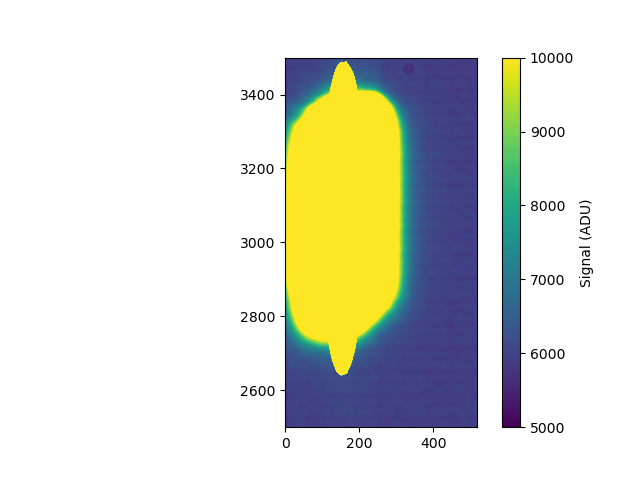
\includegraphics[width=0.32\textwidth]{figures/Rectange_Spot_Sat.png}
\caption{Example photos of the L1 cover gaps. These were covered by tape where we could safely apply it and by the black shroud.}
\label{fig:L1_Gaps}
\end{figure}

Once these were sealed, we took some initial measurements and then
started to cover the LSST Camera body with a Thorlabs blackout fabric shroud (BK5). Figure~\ref{fig:LSSTCam_config} shows the final configuration of the shroud covering the
camera.
We also found light leaks where the light cone attached to L1 was housed, and from the Utility Trunk, which were covered with shroud. Table~\ref{tab:leak_chasing} includes the observations, the corresponding measured dark currents, and comments on what changed during the chasing of the leaks.

{\small
\begin{longtable}[ht]{|l|c|l|l|l|}
\caption{Summary of the 15\,s dark exposures, the different conditions, and the resulting dark current.
Exposure ID is preceded by ``MC\_C202409".  The shroud was in place for each of these measurements.  (``Initial Covering" was just the CCOB cone and around the L1 cover.) \label{tab:leak_chasing}} \\
\hline
\textbf{Exposure} & \textbf{Dark Current} (ADU/s) & \textbf{Room Lights} &\textbf{Shutter} & \textbf{Comments} \\

\hline
\endfirsthead
\hline
%\textbf{Exposure ID} & \textbf{Dark Current (e$^-$/s)} & \textbf{Room Lights} & \textbf{Shutter} & \textbf{Comments} \\
\hline
\endhead
\hline
\endfoot
\hline
09\_000012 & 0.16 & Off & Closed & \\
09\_000018 & 0.16 & On & Closed & \\
09\_000038 & 2.94 & On & Open & Initial Covering  \\
09\_000054 & 1.34 & On & Open &  + Blanket over the FCS \\
09\_000072 & 0.41 & On & Open &  + Blanket over AND under the FCS \\
09\_000078 & 0.18 & Off & Open & + Blanket over AND under the FCS \\
10\_000031 & 0.03 & On & Open &  + Blanket over AND under the FCS + UT \\

\end{longtable}
}


\subsubsection{Filter Exchange System Autochanger light leak
masking}\label{successful-autochanger-light-leaks-masking}

A dedicated light leak study of the Filter Exchange System (FES) Autochanger (AC) was performed during Run 6 at SLAC
in summer 2023 and a localized faint light source of up to
\textasciitilde{}0.04 e$^-$/s/pix was found to be associated with the 24\,V Clean of
the AC.

In the AC this voltage is used to power some probes and all
controllers. In February 2024, as AC-1 was extracted from LSST Camera for
global maintenance, a direct investigation to localize the light
source was performed unsuccessfully. A light source in the AC
was not expected, as in the AC all controllers' LEDs have
been removed, and most electronics are in ``black boxes". Still, two small
probes, which had LEDs that could not be removed, were initially masked
by a black epoxy. As we had doubts about the quality of this masking at
IR wavelengths, we applied extra masking (aluminum black tape) on them during
the Feb 2024 maintenance (on AC 1 and 2).

At the start of Run 7 a new study of the light leak based on 900\,s
dark exposures with the shutter open and the empty frame filter in
place, showed that the AC light leaks were still present (see left-hand image of Fig.~\ref{fig:ac-light-leak}). Following this finding, a full review of all the AC hardware powered
by the 24 V dirty was performed, and a candidate was found: the encoders
of the five main motors of the AC had only partial documentation from the
vendor that did not mention the presence of LEDs. After interaction with the
vendor, the encoders were understood to contain \textasciitilde700\,nm LEDs. The hypothesis of \textasciitilde700\,nm LED sources has been
found compatible with the observation as no AC light leaks were detected
using various filters (g, r, and y ; all opaque at 700 nm ) in LSST Camera at the start of Run 7 (g, r, and y
filters). A dedicated test in Paris using an AC spare encoder and a
precision photometric set-up allowed identification of the leak in the masking of
those LEDs in the vendor packaging (see Figure \ref{fig:CoderLight}). A complementary masking method based
on a 3D printed part + tape + cable tie was qualified in Paris.  It was
found to mask the light leak and to be safe (all parts correctly secured, see Figure \ref{fig:CoderLight})).

In November 2024, we masked all the lights in the back of the Level 3 white
room (not the part containing LSST Camera) to set up a high-quality dark room
allowing a direct observation with a CMOS camera of the light leak on
the AC2 motor encoders. The level of darkness reached allowed us to
validate the quality of the light masking of the AC encoders. Notice that the
FES-prototype in Paris does not have encoders on the Online
Clamps, so we had to tune/qualify the masking of those encoders directly on the AC 2 at the summit.

For both AC 1 and 2, the encoders of the five motors with the vendor issue on
their LED masking have been successfully enveloped in a light-tight
mask (see Figure \ref{fig:CoderLight}).

We note that the AC was turned off starting on 27 September 2024 at 21:15 UTC in the
first part of Run 7. For the second part of Run 7 (i.e., after
mid-November) the AC was back on: as the AC 1 was back in LSST Camera with
the new light masks in place on the motor encorders, we were able to take a new series of
900\,s darks with the AC turned on and off, confirming that the light leak
associated with the FES was eliminated (see right-hand image of Fig.~\ref{fig:ac-light-leak}).
\begin{figure}[ht]
\centering
\begin{subfigure}{0.32\textwidth}
  \centering
  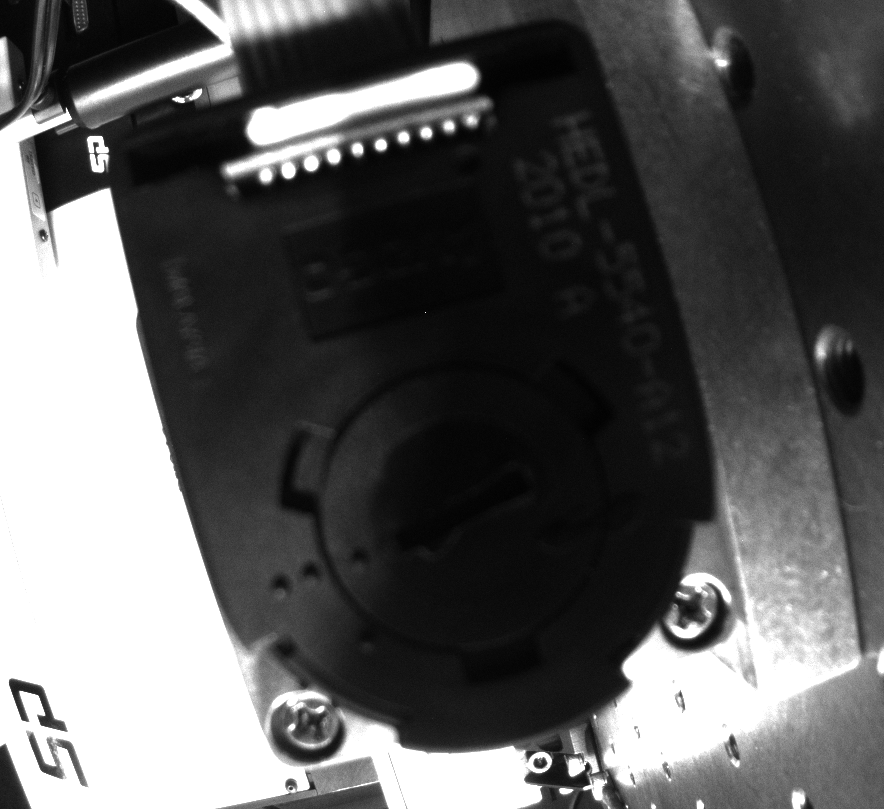
\includegraphics[width=1.0\textwidth]{figures/Codershape.png}
\end{subfigure}%
\begin{subfigure}{0.32\textwidth}
  \centering
  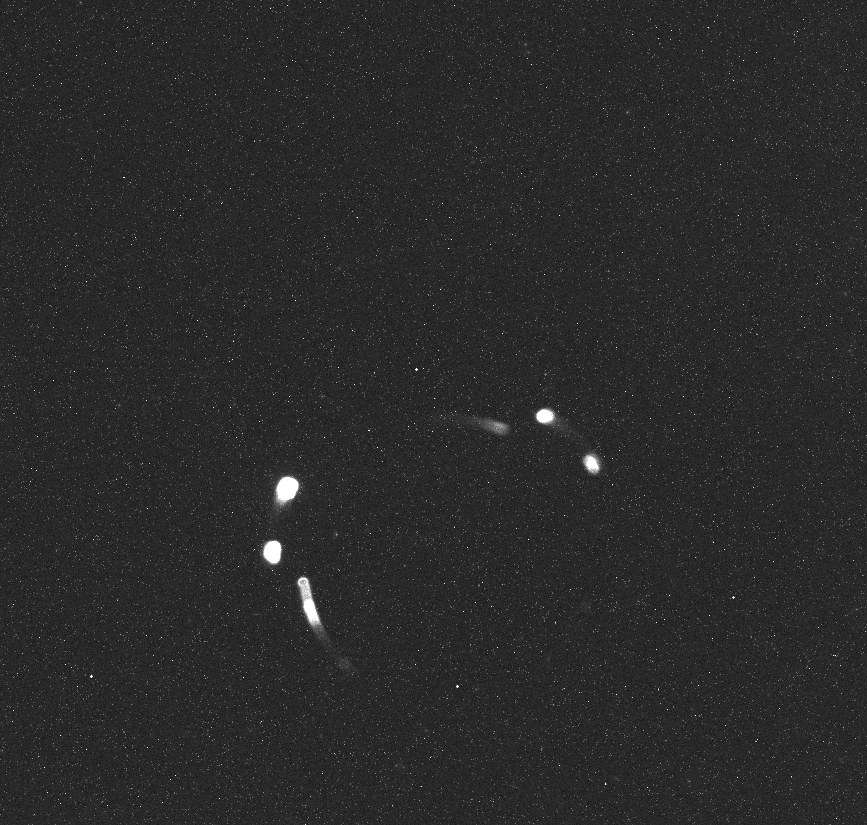
\includegraphics[width=1\textwidth]{figures/Coderligth.png}
\end{subfigure}
\begin{subfigure}{0.32\textwidth}
  \centering
  \includegraphics[width=1\textwidth]{figures/X-OnlineCoder.png}
\end{subfigure}
\caption{On the left a picture of one AC coder . In the center a 60\,s exposure , with the same coder On , light in the room off : light leak is obvious , mainly associated to holes on the top of the coder cover . On the left , the X- Online coder after masking .}
\label{fig:CoderLight}
\end{figure}

\begin{figure}[ht]
\begin{centering}
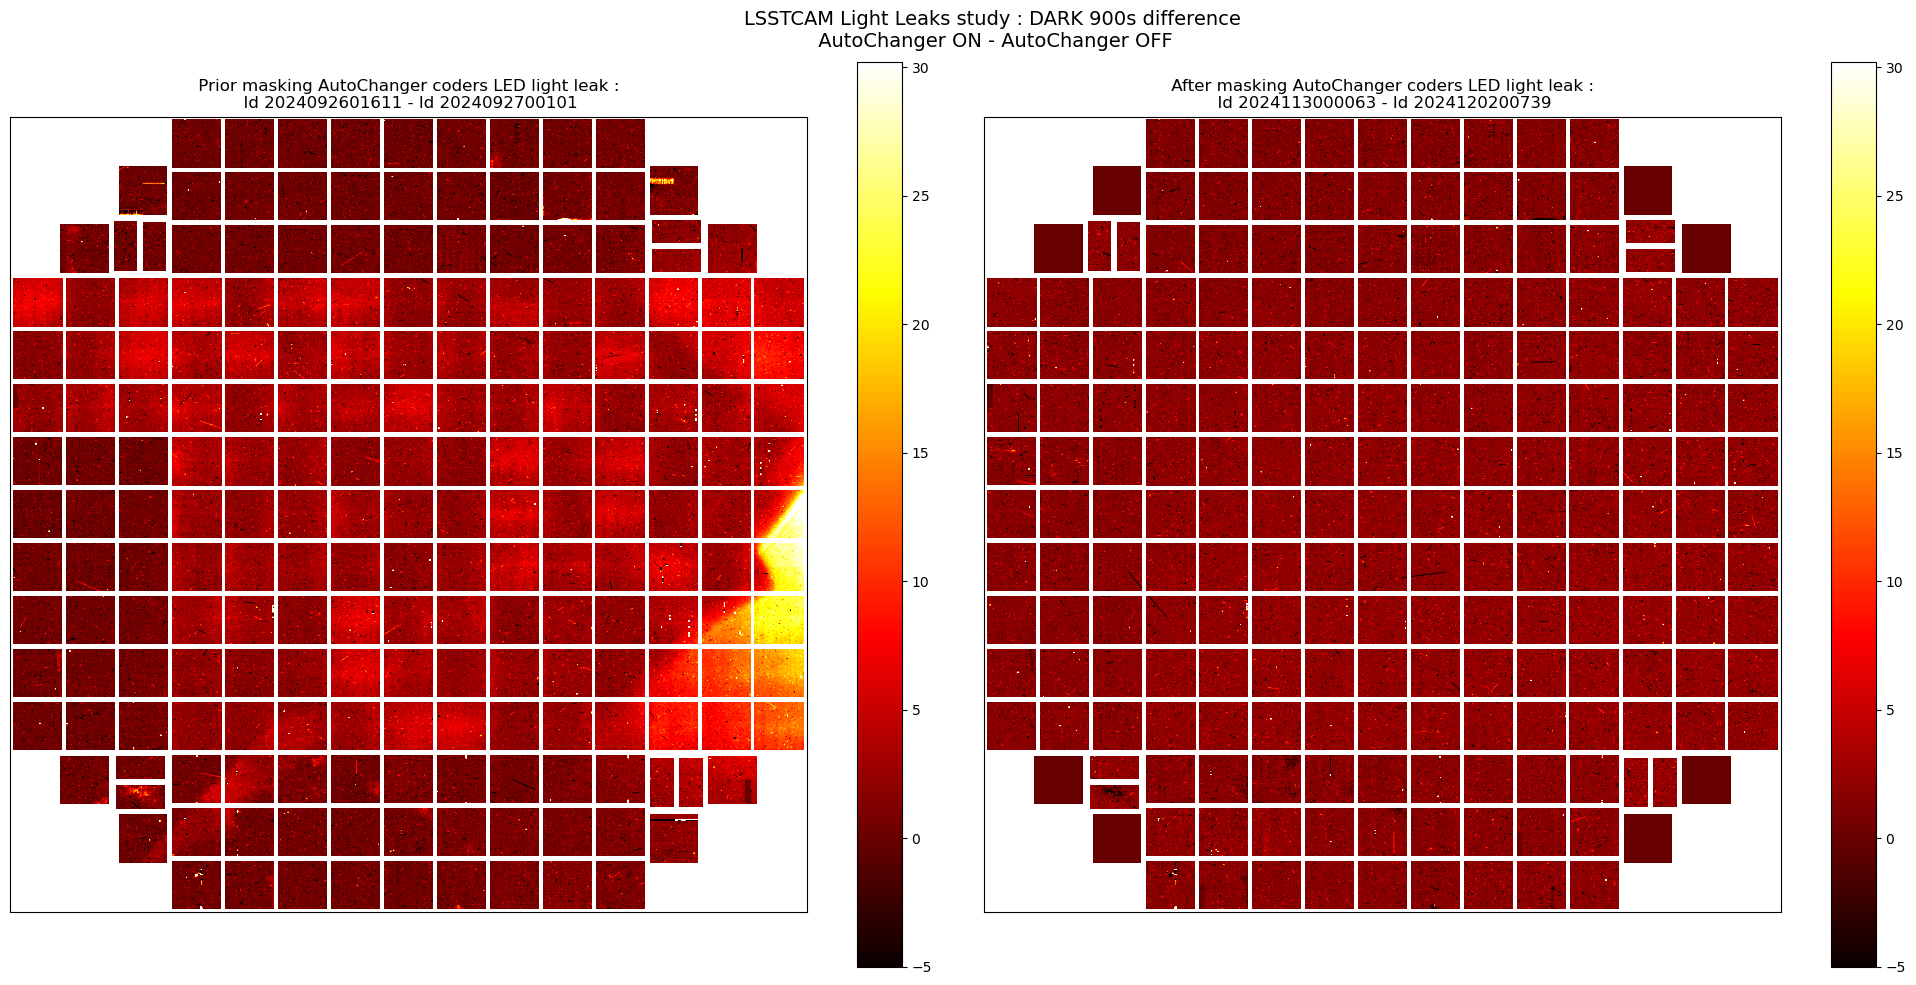
\includegraphics[width=0.8\textwidth]{figures/AC_LightLeak_study.png}
\caption{ (left) The original impact of the AC light leak on a 900\,s dark difference image (AC on minus AC off), we observe in particular a ``bright triangle" on the right of this focal plane image. We also note the presence of the persistence of \textasciitilde 10 ADU for a few sensors, the same e2v sensors than the one visible in the left figure \ref{fig:persistence-reduction}. We did not collect the exactly same condition image, a dark without the AC leak mitigation with the persistence mitigation voltages (see Sect. \ref{persistence-optimization-1}). (right) The result after masking the LEDs of the motor encoders in the AC.  No light associated with the FES is present in 900\,s dark difference image.  \label{fig:ac-light-leak}}
\end{centering}
\end{figure}

\subsection{Shutter condition impact on
darks}\label{shutter-condition-impact-on-darks}

Two runs, E1075 and E1076, were dedicated to determining the effect of the shutter on darks by keeping the shutter closed and open respectively. Figure \ref{fig:shutter-darkcurrent} shows example images of the focal plane from both of these runs. 
Figure \ref{fig:DarkCurrent_ShutterOpenvClosed} shows the difference between the shutter open and closed and how this condition affects the dark current.
No easily visible difference can be seen between the two images. This is most likely due to the shrouding of the camera (see Section \ref{light-leak-mitigation-with-shrouding-the-camera-body}) as well as the pinhole filter being in place for these runs.

\begin{figure}[ht]
\begin{centering}
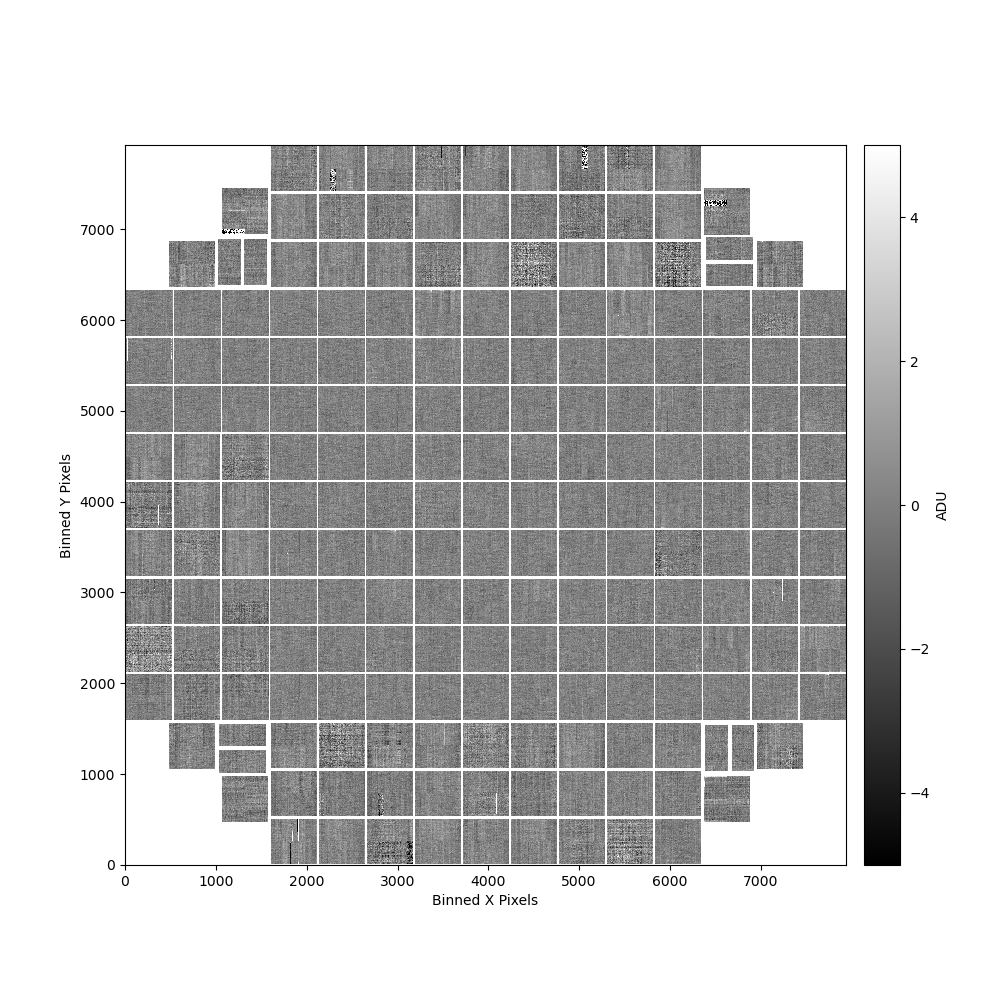
\includegraphics[width=0.48\textwidth]{figures/E1075_ShutterClosed.png}
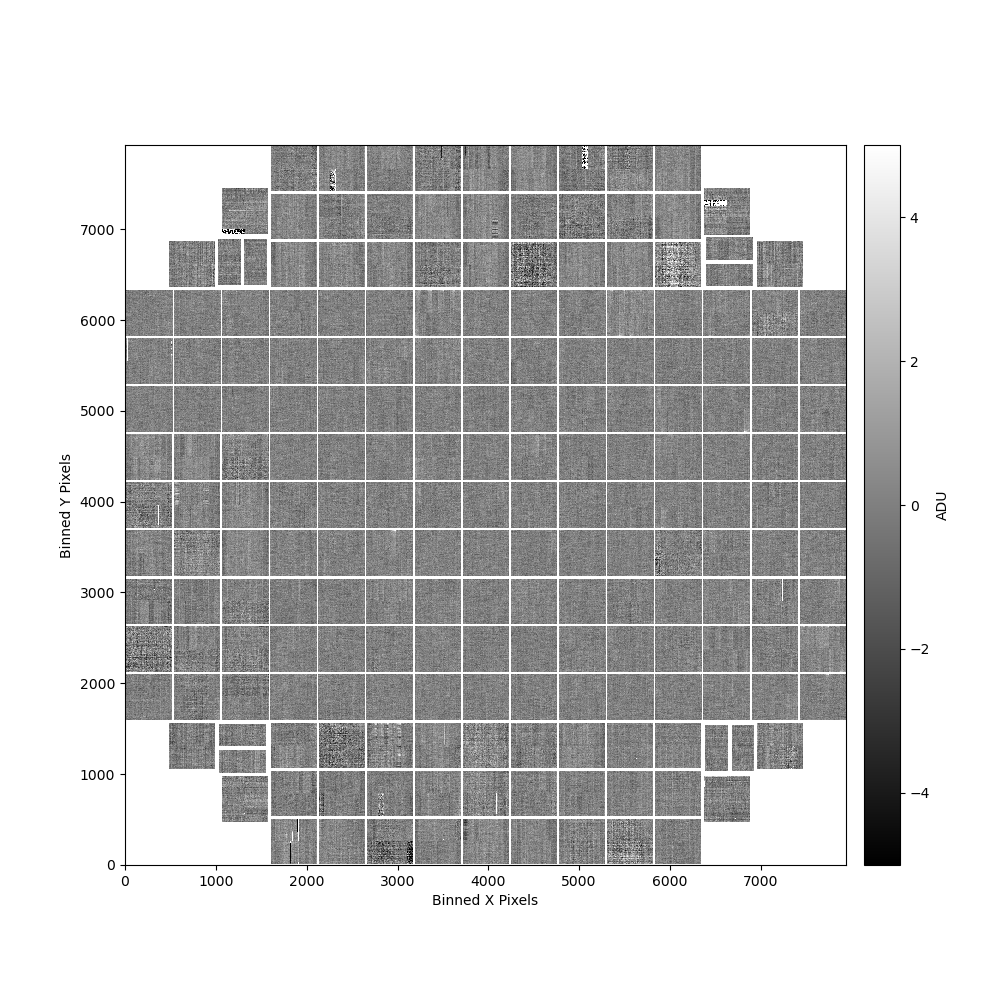
\includegraphics[width=0.48\textwidth]{figures/E1076_ShutterOpen.png}
\caption{ (left) An example image of run E1075 (shutter closed). (right) An example image of run E1076 (shutter open). If there was a light leak, we would expect to see the 21 spots of the pinhole filter. However, there is no noticeable difference between the images, insuring that our shrouding in Section \ref{light-leak-mitigation-with-shrouding-the-camera-body} is good and that the shutter being open and closed does not affect the dark current. \label{fig:shutter-darkcurrent}}
\end{centering}
\end{figure}

\begin{figure}[ht]
    \centering
    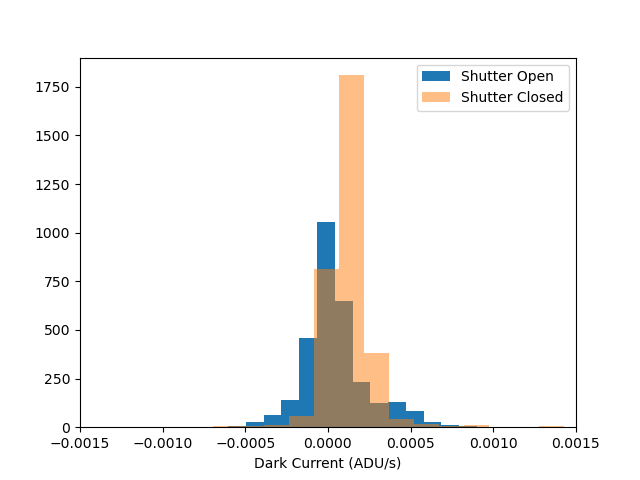
\includegraphics[width=0.5\linewidth]{figures/DarkCurrent_ShutterOpenvClosed.png}
    \caption{Histogram comparison between the dark current between the shutter being open versus closed.}
    \label{fig:DarkCurrent_ShutterOpenvClosed}
\end{figure}

\subsection{Filter condition impact on
darks}\label{filter-condition-impact-on-darks}

To investigate how the filter affects the dark measurement, we took 900 second darks with the available filters in the filter wheel: E1114 (empty filter), E1115 ($g$), E1116 ($y$), and E1117 ($r$). The heat maps of the dark currents from EO pipe can be found in Figure \ref{fig:filter-darkcurrent}. The major effect of including the filters was reducing the glow the AC (see Figure \ref{fig:ac-light-leak}). The global average of the median amplifier dark currents drop from 0.026 e-/s with the empty filter to 0.0035 e-/s for $r$, 0.0011 e-/s for $y$, and 0.00063 e-/s for $g$. The discrepancy between the filters could arise if the AC light shines more brightly in the redder wavelengths and even the IR. Unfortunately, we were not able to obtain data with the other 3 filters to confirm this.

\begin{figure}[ht]
\begin{centering}
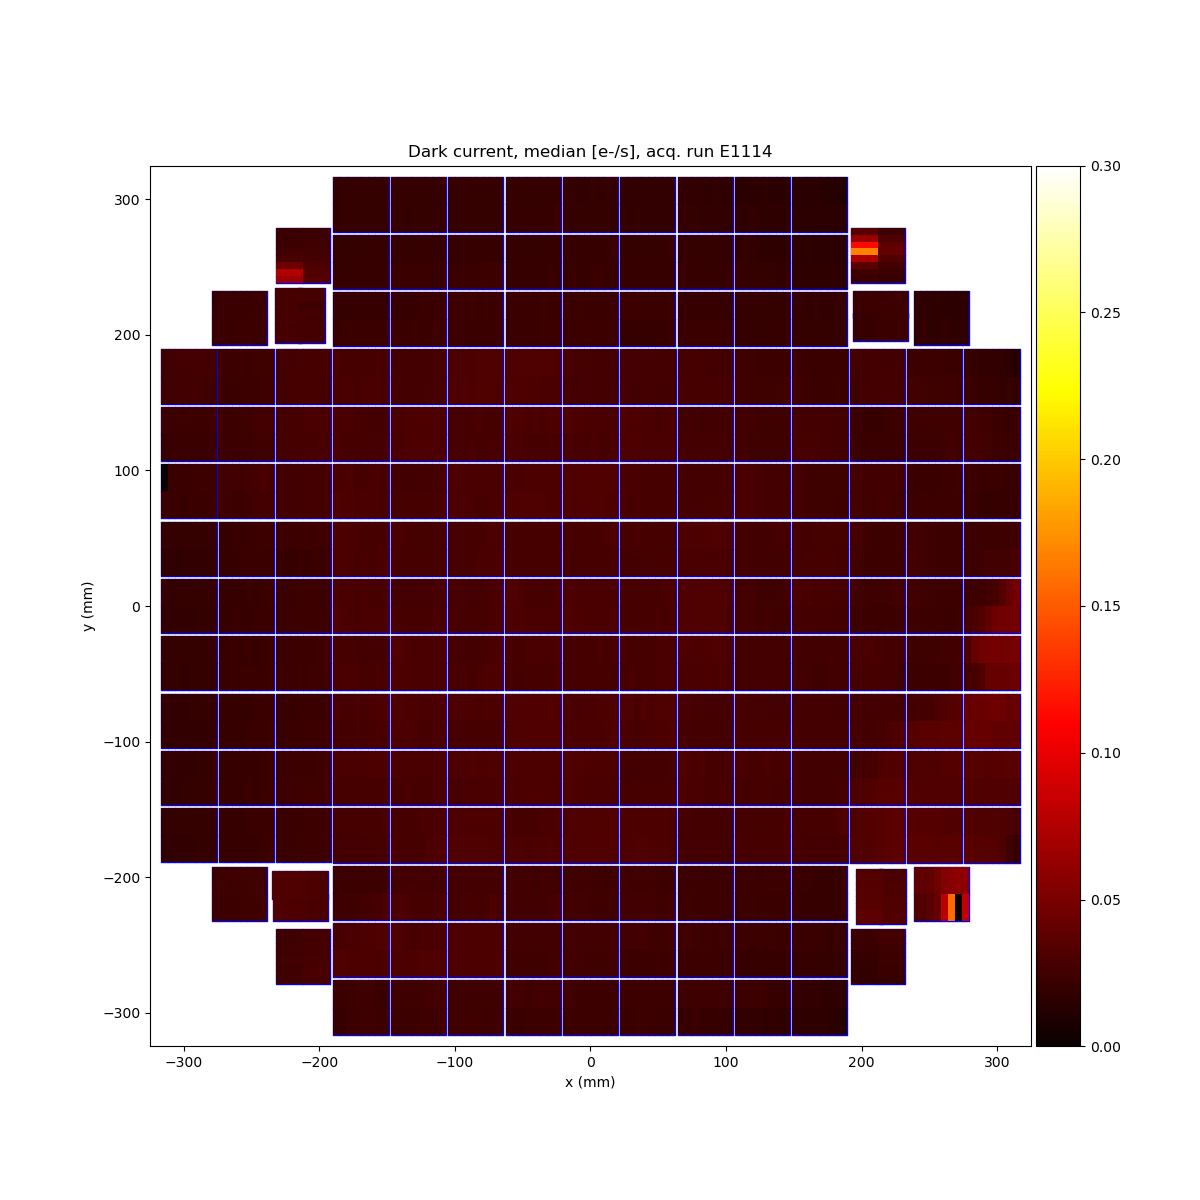
\includegraphics[width=0.48\textwidth]{figures/E1114_Empty_DarkCurrent.png}
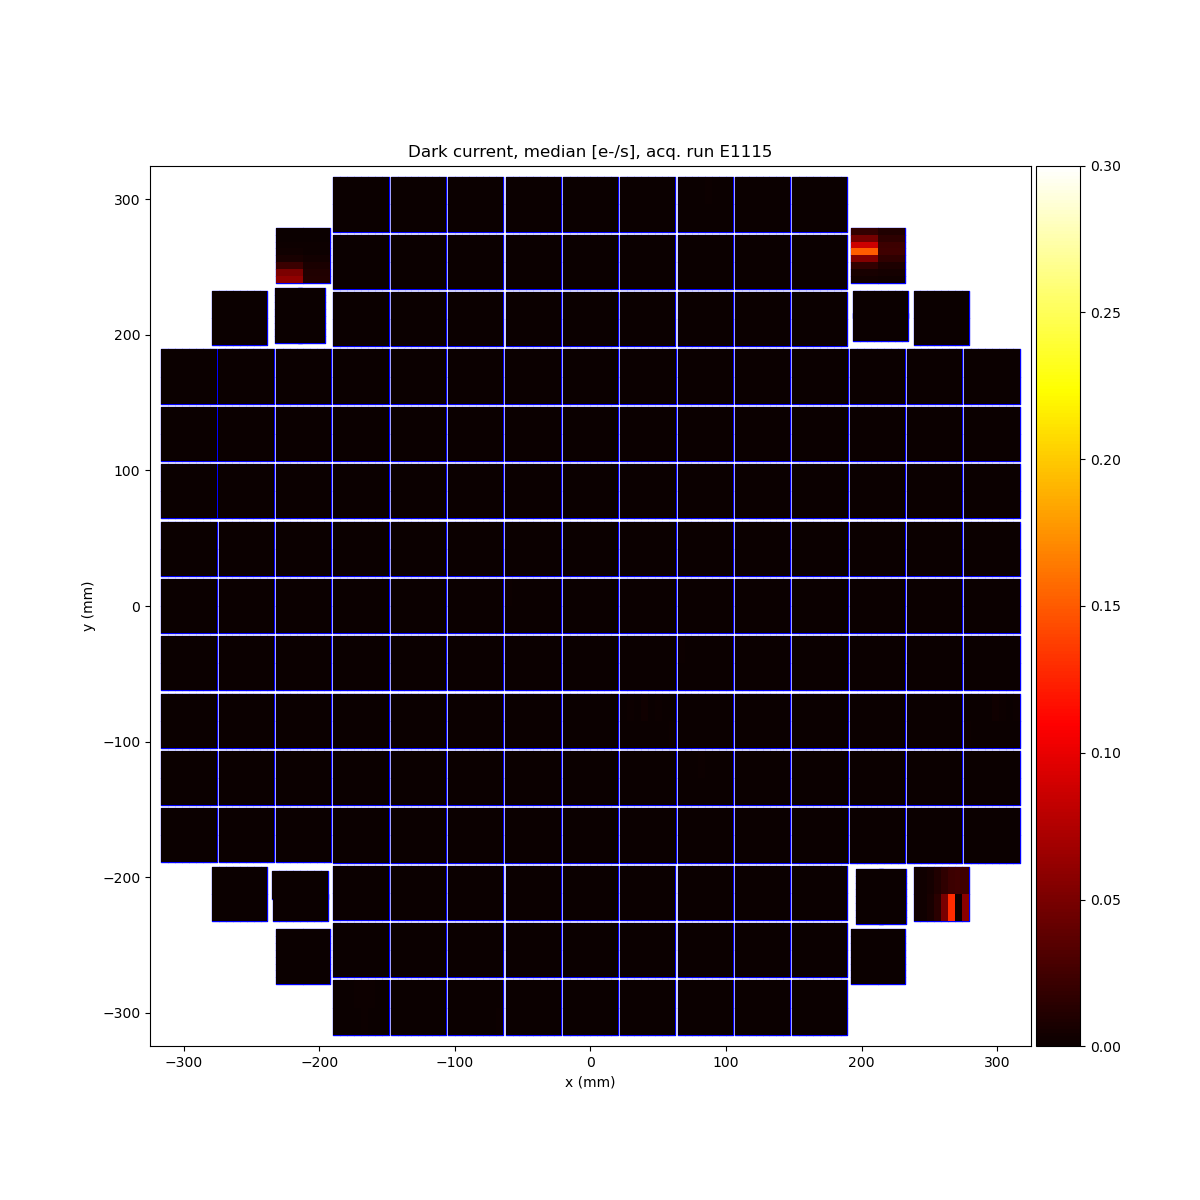
\includegraphics[width=0.48\textwidth]{figures/E1115_g_DarkCurrent.png} \\
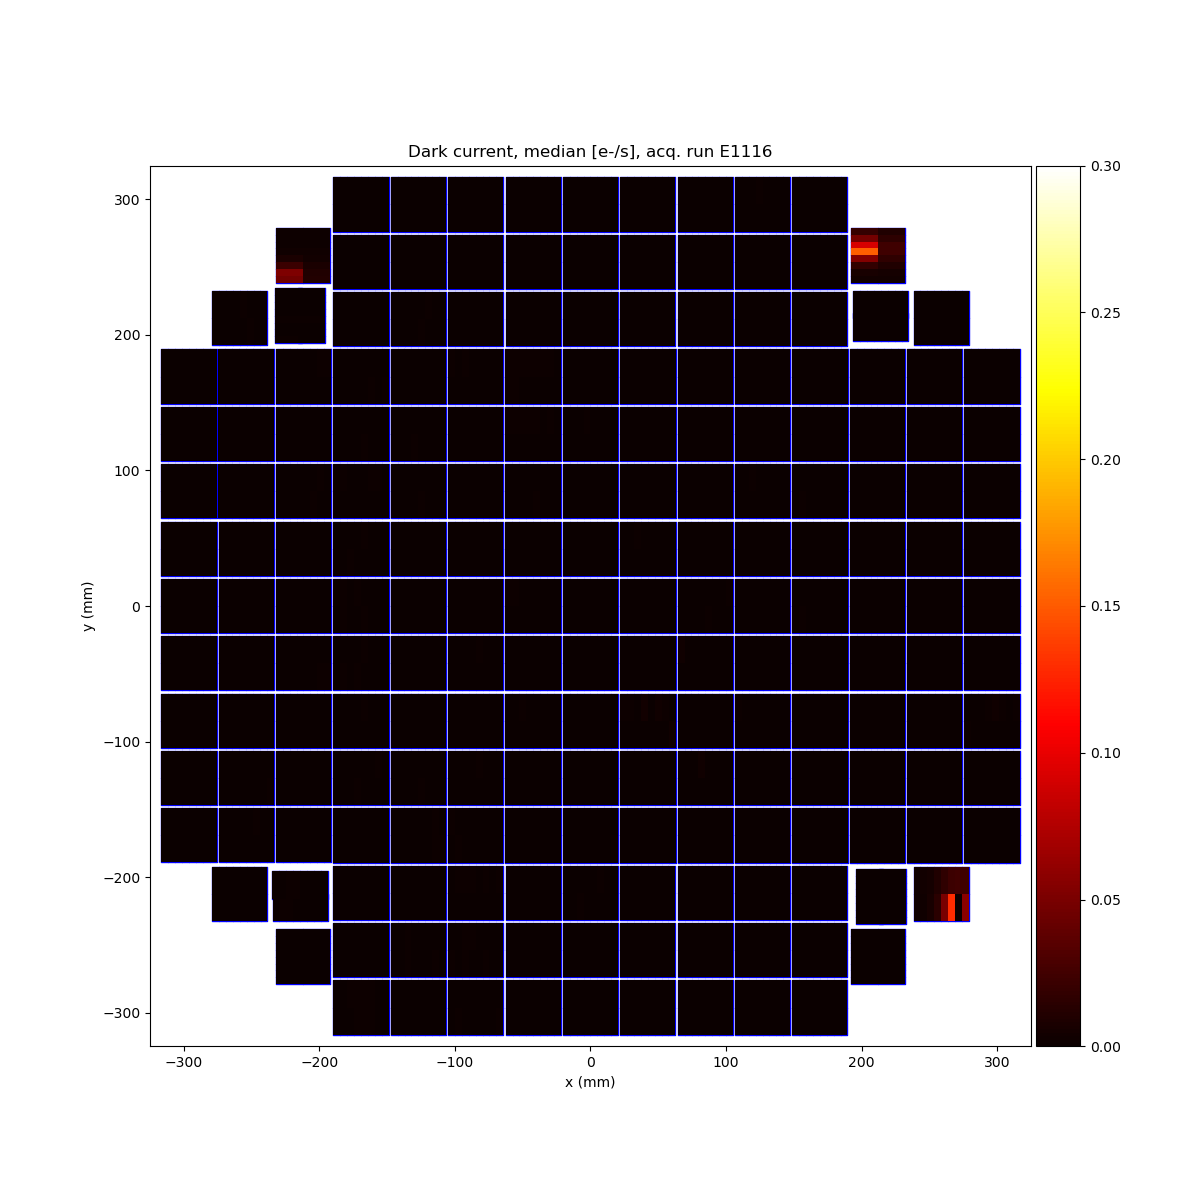
\includegraphics[width=0.48\textwidth]{figures/E1116_y_DarkCurrent.png}
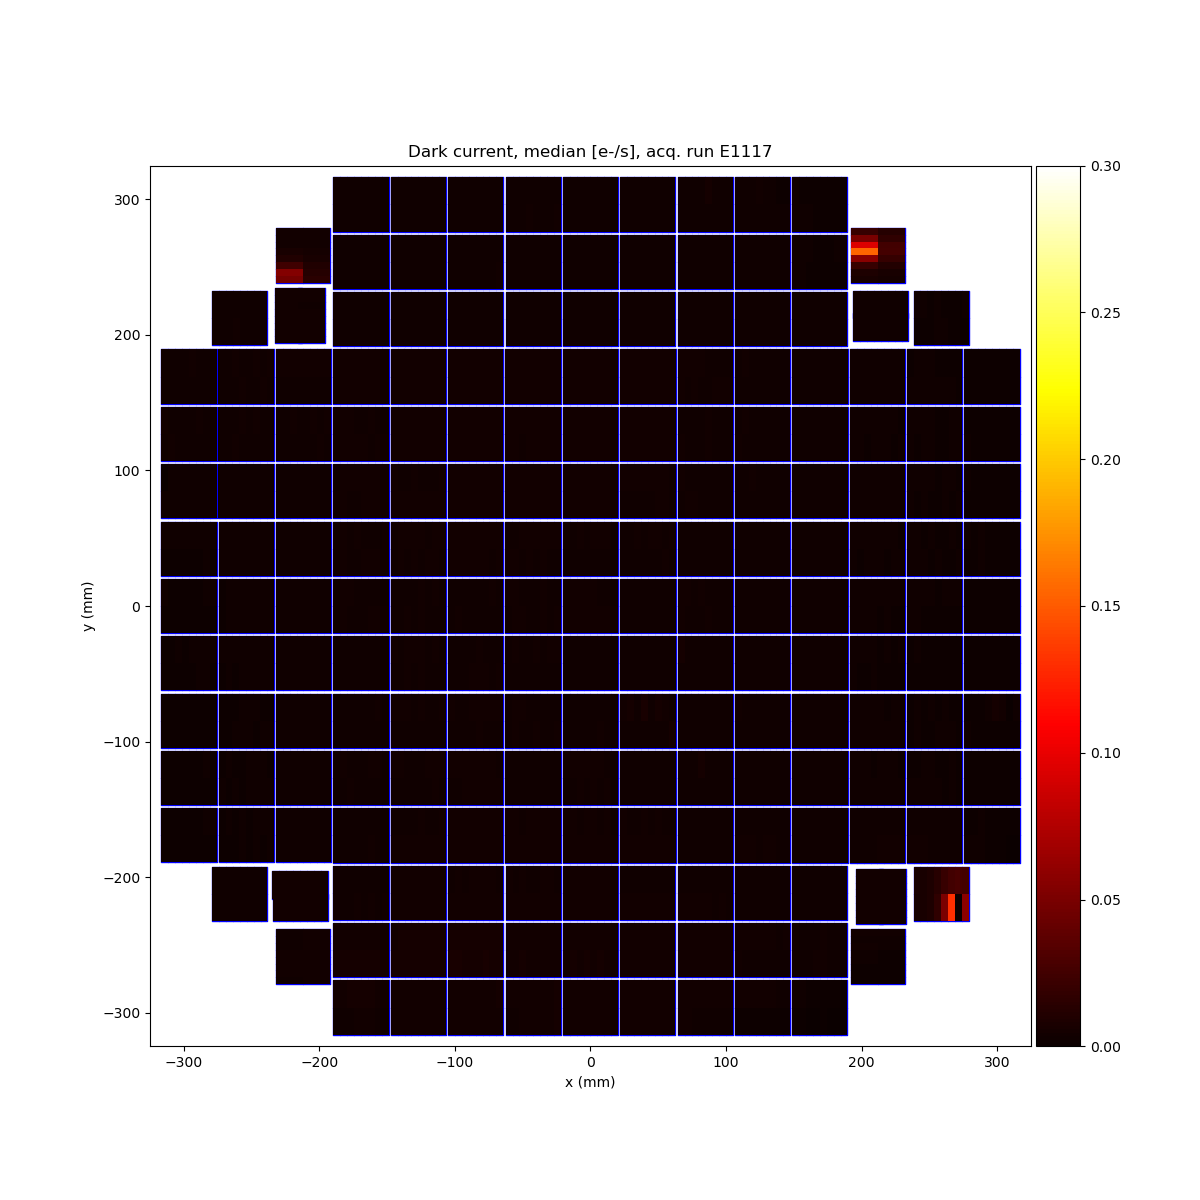
\includegraphics[width=0.48\textwidth]{figures/E1117_r_DarkCurrent.png}
\caption{ The heat map of the dark current with the empty filter installed (E1114; top left), the $g$ filter installed (E1115; top right), the $y$ filter installed (E1116; bottom left), and the $r$ filter installed (E1117; bottom right)  \label{fig:filter-darkcurrent}}
\end{centering}
\end{figure}

%\subsubsection{Final measurements of dark current}\label{final-measurements-of-dark-current}
% we don't need this since it will be compared in the following sections.

\clearpage